\documentclass[sigconf,review,10pt,acmthm=false]{acmart}
% MobiSys 2027 submission: single-blind, 12-page body limit (references + appendix excluded).

\usepackage{booktabs}
\usepackage{array}
\usepackage{amsmath,amsthm}   % acmart: do NOT load amssymb (clashes with newtx \Bbbk)
\usepackage{graphicx}
\usepackage{xcolor}
\usepackage{xspace}
\xspaceaddexceptions{\% \,}
\usepackage{algorithm}
\usepackage[noend]{algpseudocode}
\usepackage{tikz}
\usetikzlibrary{arrows.meta,positioning,calc,shapes.misc,decorations.pathreplacing,backgrounds,fit}
\usepackage{pgfplots}
\pgfplotsset{compat=1.17} % ship 1.18 on TeX Live >= 2021
\usepackage{url}
\usepackage{enumitem}
\usepackage{orcidlink}
% matured-style.tex -- shared table/plot look for the MobiSys 2027 papers (same palette as the Figure 1 comics).
% Copy into each manuscript and % matured-style.tex -- shared table/plot look for the MobiSys 2027 papers (same palette as the Figure 1 comics).
% Copy into each manuscript and % matured-style.tex -- shared table/plot look for the MobiSys 2027 papers (same palette as the Figure 1 comics).
% Copy into each manuscript and \input{matured-style} after xcolor/booktabs/pgfplots are loaded.
% Muted, print-safe colours; series also differ by marker/dash so the plots survive greyscale.
\usepackage{colortbl}
% ---- palette -----------------------------------------------------------------
\definecolor{mInk}{HTML}{2B2A29}
\definecolor{mSlate}{HTML}{5E6670}
\definecolor{mNavy}{HTML}{2F3E55}
\definecolor{mTeal}{HTML}{2F6F68}
\definecolor{mSage}{HTML}{5F8A68}
\definecolor{mOchre}{HTML}{B9873A}
\definecolor{mBrick}{HTML}{9E4A3C}
\definecolor{mPlum}{HTML}{5B3F66}
\definecolor{mHead}{HTML}{E9ECEF}   % table header fill
\definecolor{mGroup}{HTML}{F3F1EC}  % group/section row fill
\definecolor{mHiB}{HTML}{F4E3DF}    % brick tint: bad/unsafe cell
\definecolor{mHiT}{HTML}{DFEDEA}    % teal tint: good/safe cell
\definecolor{mHiO}{HTML}{F6EBD6}    % ochre tint: emphasis
% ---- tables ------------------------------------------------------------------
% \mhead   : first command of a header row  -> shaded header
% \mgroup{n}{text} : full-width shaded group label row spanning n columns
% \mbad{x} \mgood{x} \mhi{x} : tinted cells (colortbl \cellcolor)
\newcommand{\mhead}{\rowcolor{mHead}}
\newcommand{\mgroup}[2]{\rowcolor{mGroup}\multicolumn{#1}{@{}l}{\textit{#2}}\\}
\newcommand{\mbad}[1]{\cellcolor{mHiB}#1}
\newcommand{\mgood}[1]{\cellcolor{mHiT}#1}
\newcommand{\mhi}[1]{\cellcolor{mHiO}#1}
\newcommand{\mtab}{\footnotesize\setlength{\tabcolsep}{3.6pt}\renewcommand{\arraystretch}{1.05}}
\setlength{\aboverulesep}{0.25ex}\setlength{\belowrulesep}{0.4ex}
\setlength{\heavyrulewidth}{0.08em}\setlength{\lightrulewidth}{0.05em}
% ---- plots -------------------------------------------------------------------
\pgfplotscreateplotcyclelist{matured}{%
  {mBrick,mark=*,mark size=1.4pt},
  {mTeal,mark=square*,mark size=1.3pt},
  {mOchre,mark=triangle*,mark size=1.7pt},
  {mNavy,mark=diamond*,mark size=1.7pt},
  {mSage,mark=pentagon*,mark size=1.5pt},
  {mPlum,mark=o,mark size=1.4pt}}
\pgfplotscreateplotcyclelist{maturedbars}{%
  {fill=mBrick,draw=mInk!75},{fill=mTeal,draw=mInk!75},{fill=mOchre,draw=mInk!75},
  {fill=mNavy,draw=mInk!75},{fill=mSage,draw=mInk!75},{fill=mPlum,draw=mInk!75}}
\pgfplotsset{
  matured/.style={
    cycle list name=matured,
    every axis plot/.append style={line width=0.9pt},
    axis x line*=bottom, axis y line*=left,
    axis line style={draw=mSlate!80, line width=0.5pt},
    every tick/.style={draw=mSlate!80, line width=0.4pt}, tick align=outside, major tick length=2pt,
    ymajorgrids, major grid style={draw=mSlate!18, line width=0.35pt},
    tick label style={font=\footnotesize, text=mInk},
    label style={font=\footnotesize, text=mInk},
    title style={font=\footnotesize\bfseries, text=mInk, yshift=-1ex},
    legend style={font=\footnotesize, draw=none, fill=white, fill opacity=0.85, text opacity=1,
                  legend cell align=left, column sep=4pt},
    legend image post style={line width=0.9pt},
    error bars/error bar style={line width=0.5pt},
    error bars/error mark options={rotate=90, mark size=1.4pt, line width=0.5pt},
  },
  maturedbar/.style={matured, ybar, bar width=5pt, enlarge x limits=0.12, cycle list name=maturedbars,
    every axis plot/.append style={line width=0.4pt}},
}
 after xcolor/booktabs/pgfplots are loaded.
% Muted, print-safe colours; series also differ by marker/dash so the plots survive greyscale.
\usepackage{colortbl}
% ---- palette -----------------------------------------------------------------
\definecolor{mInk}{HTML}{2B2A29}
\definecolor{mSlate}{HTML}{5E6670}
\definecolor{mNavy}{HTML}{2F3E55}
\definecolor{mTeal}{HTML}{2F6F68}
\definecolor{mSage}{HTML}{5F8A68}
\definecolor{mOchre}{HTML}{B9873A}
\definecolor{mBrick}{HTML}{9E4A3C}
\definecolor{mPlum}{HTML}{5B3F66}
\definecolor{mHead}{HTML}{E9ECEF}   % table header fill
\definecolor{mGroup}{HTML}{F3F1EC}  % group/section row fill
\definecolor{mHiB}{HTML}{F4E3DF}    % brick tint: bad/unsafe cell
\definecolor{mHiT}{HTML}{DFEDEA}    % teal tint: good/safe cell
\definecolor{mHiO}{HTML}{F6EBD6}    % ochre tint: emphasis
% ---- tables ------------------------------------------------------------------
% \mhead   : first command of a header row  -> shaded header
% \mgroup{n}{text} : full-width shaded group label row spanning n columns
% \mbad{x} \mgood{x} \mhi{x} : tinted cells (colortbl \cellcolor)
\newcommand{\mhead}{\rowcolor{mHead}}
\newcommand{\mgroup}[2]{\rowcolor{mGroup}\multicolumn{#1}{@{}l}{\textit{#2}}\\}
\newcommand{\mbad}[1]{\cellcolor{mHiB}#1}
\newcommand{\mgood}[1]{\cellcolor{mHiT}#1}
\newcommand{\mhi}[1]{\cellcolor{mHiO}#1}
\newcommand{\mtab}{\footnotesize\setlength{\tabcolsep}{3.6pt}\renewcommand{\arraystretch}{1.05}}
\setlength{\aboverulesep}{0.25ex}\setlength{\belowrulesep}{0.4ex}
\setlength{\heavyrulewidth}{0.08em}\setlength{\lightrulewidth}{0.05em}
% ---- plots -------------------------------------------------------------------
\pgfplotscreateplotcyclelist{matured}{%
  {mBrick,mark=*,mark size=1.4pt},
  {mTeal,mark=square*,mark size=1.3pt},
  {mOchre,mark=triangle*,mark size=1.7pt},
  {mNavy,mark=diamond*,mark size=1.7pt},
  {mSage,mark=pentagon*,mark size=1.5pt},
  {mPlum,mark=o,mark size=1.4pt}}
\pgfplotscreateplotcyclelist{maturedbars}{%
  {fill=mBrick,draw=mInk!75},{fill=mTeal,draw=mInk!75},{fill=mOchre,draw=mInk!75},
  {fill=mNavy,draw=mInk!75},{fill=mSage,draw=mInk!75},{fill=mPlum,draw=mInk!75}}
\pgfplotsset{
  matured/.style={
    cycle list name=matured,
    every axis plot/.append style={line width=0.9pt},
    axis x line*=bottom, axis y line*=left,
    axis line style={draw=mSlate!80, line width=0.5pt},
    every tick/.style={draw=mSlate!80, line width=0.4pt}, tick align=outside, major tick length=2pt,
    ymajorgrids, major grid style={draw=mSlate!18, line width=0.35pt},
    tick label style={font=\footnotesize, text=mInk},
    label style={font=\footnotesize, text=mInk},
    title style={font=\footnotesize\bfseries, text=mInk, yshift=-1ex},
    legend style={font=\footnotesize, draw=none, fill=white, fill opacity=0.85, text opacity=1,
                  legend cell align=left, column sep=4pt},
    legend image post style={line width=0.9pt},
    error bars/error bar style={line width=0.5pt},
    error bars/error mark options={rotate=90, mark size=1.4pt, line width=0.5pt},
  },
  maturedbar/.style={matured, ybar, bar width=5pt, enlarge x limits=0.12, cycle list name=maturedbars,
    every axis plot/.append style={line width=0.4pt}},
}
 after xcolor/booktabs/pgfplots are loaded.
% Muted, print-safe colours; series also differ by marker/dash so the plots survive greyscale.
\usepackage{colortbl}
% ---- palette -----------------------------------------------------------------
\definecolor{mInk}{HTML}{2B2A29}
\definecolor{mSlate}{HTML}{5E6670}
\definecolor{mNavy}{HTML}{2F3E55}
\definecolor{mTeal}{HTML}{2F6F68}
\definecolor{mSage}{HTML}{5F8A68}
\definecolor{mOchre}{HTML}{B9873A}
\definecolor{mBrick}{HTML}{9E4A3C}
\definecolor{mPlum}{HTML}{5B3F66}
\definecolor{mHead}{HTML}{E9ECEF}   % table header fill
\definecolor{mGroup}{HTML}{F3F1EC}  % group/section row fill
\definecolor{mHiB}{HTML}{F4E3DF}    % brick tint: bad/unsafe cell
\definecolor{mHiT}{HTML}{DFEDEA}    % teal tint: good/safe cell
\definecolor{mHiO}{HTML}{F6EBD6}    % ochre tint: emphasis
% ---- tables ------------------------------------------------------------------
% \mhead   : first command of a header row  -> shaded header
% \mgroup{n}{text} : full-width shaded group label row spanning n columns
% \mbad{x} \mgood{x} \mhi{x} : tinted cells (colortbl \cellcolor)
\newcommand{\mhead}{\rowcolor{mHead}}
\newcommand{\mgroup}[2]{\rowcolor{mGroup}\multicolumn{#1}{@{}l}{\textit{#2}}\\}
\newcommand{\mbad}[1]{\cellcolor{mHiB}#1}
\newcommand{\mgood}[1]{\cellcolor{mHiT}#1}
\newcommand{\mhi}[1]{\cellcolor{mHiO}#1}
\newcommand{\mtab}{\footnotesize\setlength{\tabcolsep}{3.6pt}\renewcommand{\arraystretch}{1.05}}
\setlength{\aboverulesep}{0.25ex}\setlength{\belowrulesep}{0.4ex}
\setlength{\heavyrulewidth}{0.08em}\setlength{\lightrulewidth}{0.05em}
% ---- plots -------------------------------------------------------------------
\pgfplotscreateplotcyclelist{matured}{%
  {mBrick,mark=*,mark size=1.4pt},
  {mTeal,mark=square*,mark size=1.3pt},
  {mOchre,mark=triangle*,mark size=1.7pt},
  {mNavy,mark=diamond*,mark size=1.7pt},
  {mSage,mark=pentagon*,mark size=1.5pt},
  {mPlum,mark=o,mark size=1.4pt}}
\pgfplotscreateplotcyclelist{maturedbars}{%
  {fill=mBrick,draw=mInk!75},{fill=mTeal,draw=mInk!75},{fill=mOchre,draw=mInk!75},
  {fill=mNavy,draw=mInk!75},{fill=mSage,draw=mInk!75},{fill=mPlum,draw=mInk!75}}
\pgfplotsset{
  matured/.style={
    cycle list name=matured,
    every axis plot/.append style={line width=0.9pt},
    axis x line*=bottom, axis y line*=left,
    axis line style={draw=mSlate!80, line width=0.5pt},
    every tick/.style={draw=mSlate!80, line width=0.4pt}, tick align=outside, major tick length=2pt,
    ymajorgrids, major grid style={draw=mSlate!18, line width=0.35pt},
    tick label style={font=\footnotesize, text=mInk},
    label style={font=\footnotesize, text=mInk},
    title style={font=\footnotesize\bfseries, text=mInk, yshift=-1ex},
    legend style={font=\footnotesize, draw=none, fill=white, fill opacity=0.85, text opacity=1,
                  legend cell align=left, column sep=4pt},
    legend image post style={line width=0.9pt},
    error bars/error bar style={line width=0.5pt},
    error bars/error mark options={rotate=90, mark size=1.4pt, line width=0.5pt},
  },
  maturedbar/.style={matured, ybar, bar width=5pt, enlarge x limits=0.12, cycle list name=maturedbars,
    every axis plot/.append style={line width=0.4pt}},
}
 % shared muted palette, compact tables, pgfplots styles
\emergencystretch=1.5em

% names and notation
\newcommand{\sys}{\textsc{ResidueDroid}\xspace}
\newcommand{\lab}{\textsc{ResidueLab}\xspace}
\newcommand{\icon}[2][1.0em]{\raisebox{-0.2em}{\includegraphics[height=#1]{figures/icons/#2}}}
\newcommand{\ep}{\epsilon}
\newcommand{\vname}[1]{\textsf{#1}}

\theoremstyle{plain}
\newtheorem{theorem}{Theorem}
\newtheorem{proposition}[theorem]{Proposition}
\newtheorem{lemma}[theorem]{Lemma}
\newtheorem{corollary}{Corollary}
\theoremstyle{definition}
\newtheorem{definition}{Definition}
\newtheorem{assumption}{Assumption}

% generated by artifact/scripts/render.py; do not edit
\newcommand{\acraApps}{16\xspace}
\newcommand{\acraExcluded}{0\xspace}
\newcommand{\acraFenceBlockLogged}{30/30\xspace}
\newcommand{\acraFenceCtl}{30/30\xspace}
\newcommand{\acraFenceLeak}{0/30\xspace}
\newcommand{\acraFenceReb}{0/10\xspace}
\newcommand{\acraFenceRebCtl}{10/10\xspace}
\newcommand{\acraJobGoneReb}{40/40\xspace}
\newcommand{\acraLatencyMed}{0.2\xspace}
\newcommand{\acraLogged}{160\xspace}
\newcommand{\acraStockCtl}{30/30\xspace}
\newcommand{\acraStockLeak}{30/30\xspace}
\newcommand{\acraStockReb}{0/10\xspace}
\newcommand{\acraStockRebCtl}{10/10\xspace}
\newcommand{\acraValid}{160\xspace}
\newcommand{\benchN}{8550\xspace}
\newcommand{\benchReps}{3\xspace}
\newcommand{\cancelNetPct}{100\xspace}
\newcommand{\candConsentHiN}{18\xspace}
\newcommand{\candConsentLoN}{8\xspace}
\newcommand{\cmaxMedianMs}{635\xspace}
\newcommand{\convNetPct}{100\xspace}
\newcommand{\convNoLineagePct}{14\xspace}
\newcommand{\convOtherLifeK}{1\xspace}
\newcommand{\convOtherLifeN}{1{,}000\xspace}
\newcommand{\convRacePct}{50\xspace}
\newcommand{\convTOneLifePct}{100\xspace}
\newcommand{\convTOnePct}{72\xspace}
\newcommand{\convViolPct}{26\xspace}
\newcommand{\corpusN}{360\xspace}
\newcommand{\crashKills}{100\xspace}
\newcommand{\crashOrphA}{0\xspace}
\newcommand{\crashOrphB}{86\xspace}
\newcommand{\crashOrphBPct}{86\xspace}
\newcommand{\defOtherConnStop}{44\xspace}
\newcommand{\defOtherReb}{44\xspace}
\newcommand{\defOtherTT}{44\xspace}
\newcommand{\defOtherTsix}{13\xspace}
\newcommand{\deficitCancelPct}{0.1\xspace}
\newcommand{\deficitConvPct}{1.1\xspace}
\newcommand{\deficitEgressPct}{0.0\xspace}
\newcommand{\deficitEnqueuePct}{0.0\xspace}
\newcommand{\deficitJobstartPct}{0.3\xspace}
\newcommand{\deficitNonePct}{0.0\xspace}
\newcommand{\deficitRdPct}{0.0\xspace}
\newcommand{\deficitRdbPct}{0.1\xspace}
\newcommand{\deficitTaintPct}{55.6\xspace}
\newcommand{\deficitVolatilePct}{0.6\xspace}
\newcommand{\eeEgressMs}{11.1\xspace}
\newcommand{\eeNoneMs}{12.4\xspace}
\newcommand{\eeRdMs}{13.1\xspace}
\newcommand{\egressTFivePct}{86\xspace}
\newcommand{\egressTOnePct}{71\xspace}
\newcommand{\eligibleN}{2442\xspace}
\newcommand{\enqueueFstopPct}{40\xspace}
\newcommand{\enqueueLifePct}{100\xspace}
\newcommand{\extrasDelta}{52\xspace}
\newcommand{\fenceConvUs}{579\xspace}
\newcommand{\fenceNoneUs}{480\xspace}
\newcommand{\fenceRdUs}{583\xspace}
\newcommand{\impLoc}{1{,}230\xspace}
\newcommand{\insDeltaUs}{11\xspace}
\newcommand{\insLabUs}{652\xspace}
\newcommand{\insNoUs}{641\xspace}
\newcommand{\jobEntries}{216\xspace}
\newcommand{\jobEntriesApp}{170\xspace}
\newcommand{\jobstartNetPct}{99\xspace}
\newcommand{\lcForcestopN}{50\xspace}
\newcommand{\lcKillN}{50\xspace}
\newcommand{\lcPendingN}{50\xspace}
\newcommand{\lcRebootN}{50\xspace}
\newcommand{\lcRevokeN}{50\xspace}
\newcommand{\lcTrials}{250\xspace}
\newcommand{\matomoApps}{2\xspace}
\newcommand{\medianDepth}{5\xspace}
\newcommand{\microAvd}{B\xspace}
\newcommand{\minTrialsPerSched}{50\xspace}
\newcommand{\nCmax}{150\xspace}
\newcommand{\nInflightTT}{150\xspace}
\newcommand{\nInvalid}{55\xspace}
\newcommand{\nSubmissions}{94{,}568\xspace}
\newcommand{\nTrialsTotal}{825\xspace}
\newcommand{\nTrialsValid}{700\xspace}
\newcommand{\nValidAll}{770\xspace}
\newcommand{\nValidUnused}{70\xspace}
\newcommand{\noneLifePct}{100\xspace}
\newcommand{\noserFivePct}{46\xspace}
\newcommand{\noserOnePct}{33\xspace}
\newcommand{\noserZeroPct}{39\xspace}
\newcommand{\opaqueTrials}{700\xspace}
\newcommand{\opaqueUnknownSubs}{2808\xspace}
\newcommand{\outstandingRd}{500\xspace}
\newcommand{\outstandingSubs}{2500\xspace}
\newcommand{\pctAlarmAll}{62\xspace}
\newcommand{\pctCandConsentHi}{5\xspace}
\newcommand{\pctCandConsentLo}{2\xspace}
\newcommand{\pctCandHi}{17\xspace}
\newcommand{\pctCandLo}{6\xspace}
\newcommand{\pctConsentRand}{14\xspace}
\newcommand{\pctConsentTrack}{38\xspace}
\newcommand{\pctNativeAll}{69\xspace}
\newcommand{\pctNetAll}{93\xspace}
\newcommand{\pctPersistAll}{38\xspace}
\newcommand{\pctPollStop}{20\xspace}
\newcommand{\pctSdkRand}{5\xspace}
\newcommand{\pctSdkTrack}{32\xspace}
\newcommand{\predAgree}{149\xspace}
\newcommand{\predMaxAbsErr}{0.06\xspace}
\newcommand{\predN}{150\xspace}
\newcommand{\randN}{300\xspace}
\newcommand{\rdFpBlocks}{0\xspace}
\newcommand{\rdItems}{0\xspace}
\newcommand{\rdOpaqueUnknown}{0\xspace}
\newcommand{\rdStressViol}{0\xspace}
\newcommand{\rdTenantTrials}{3500\xspace}
\newcommand{\rdUnmedPct}{78\xspace}
\newcommand{\stressRounds}{300\xspace}
\newcommand{\subAlarmManagerConvDefPct}{44\xspace}
\newcommand{\subAlarmManagerConvForcestop}{5\xspace}
\newcommand{\subAlarmManagerConvKill}{20\xspace}
\newcommand{\subAlarmManagerConvPending}{20\xspace}
\newcommand{\subAlarmManagerConvReboot}{0\xspace}
\newcommand{\subAlarmManagerConvTNinePct}{0\xspace}
\newcommand{\subAlarmManagerInvalid}{0\xspace}
\newcommand{\subAlarmManagerLogged}{80\xspace}
\newcommand{\subAlarmManagerMinPerSched}{20\xspace}
\newcommand{\subAlarmManagerNoneDefPct}{49\xspace}
\newcommand{\subAlarmManagerNoneForcestop}{4\xspace}
\newcommand{\subAlarmManagerNoneKill}{100\xspace}
\newcommand{\subAlarmManagerNonePending}{100\xspace}
\newcommand{\subAlarmManagerNoneReboot}{0\xspace}
\newcommand{\subAlarmManagerNoneTNinePct}{51\xspace}
\newcommand{\subAlarmManagerRdDefPct}{31\xspace}
\newcommand{\subAlarmManagerRdForcestop}{0\xspace}
\newcommand{\subAlarmManagerRdItems}{0\xspace}
\newcommand{\subAlarmManagerRdKill}{0\xspace}
\newcommand{\subAlarmManagerRdPending}{0\xspace}
\newcommand{\subAlarmManagerRdReboot}{0\xspace}
\newcommand{\subAlarmManagerRdTNinePct}{69\xspace}
\newcommand{\subAlarmManagerRdTT}{400\xspace}
\newcommand{\subAlarmManagerTrials}{80\xspace}
\newcommand{\subWorkManagerConvDefPct}{0\xspace}
\newcommand{\subWorkManagerConvForcestop}{20\xspace}
\newcommand{\subWorkManagerConvKill}{20\xspace}
\newcommand{\subWorkManagerConvPending}{20\xspace}
\newcommand{\subWorkManagerConvReboot}{20\xspace}
\newcommand{\subWorkManagerConvTNinePct}{0\xspace}
\newcommand{\subWorkManagerInvalid}{2\xspace}
\newcommand{\subWorkManagerLogged}{80\xspace}
\newcommand{\subWorkManagerMinPerSched}{19\xspace}
\newcommand{\subWorkManagerNoneDefPct}{0\xspace}
\newcommand{\subWorkManagerNoneForcestop}{100\xspace}
\newcommand{\subWorkManagerNoneKill}{100\xspace}
\newcommand{\subWorkManagerNonePending}{100\xspace}
\newcommand{\subWorkManagerNoneReboot}{100\xspace}
\newcommand{\subWorkManagerNoneTNinePct}{100\xspace}
\newcommand{\subWorkManagerRdDefPct}{0\xspace}
\newcommand{\subWorkManagerRdForcestop}{0\xspace}
\newcommand{\subWorkManagerRdItems}{0\xspace}
\newcommand{\subWorkManagerRdKill}{0\xspace}
\newcommand{\subWorkManagerRdPending}{0\xspace}
\newcommand{\subWorkManagerRdReboot}{0\xspace}
\newcommand{\subWorkManagerRdTNinePct}{100\xspace}
\newcommand{\subWorkManagerRdTT}{390\xspace}
\newcommand{\subWorkManagerTrials}{78\xspace}
\newcommand{\tNineCancelPct}{0\xspace}
\newcommand{\tNineConvPct}{0\xspace}
\newcommand{\tNineEgressPct}{100\xspace}
\newcommand{\tNineEnqueuePct}{80\xspace}
\newcommand{\tNineJobstartPct}{0\xspace}
\newcommand{\tNineNonePct}{100\xspace}
\newcommand{\tNineRdPct}{100\xspace}
\newcommand{\tNineRdbPct}{100\xspace}
\newcommand{\tNineTaintPct}{100\xspace}
\newcommand{\tNineVolatilePct}{100\xspace}
\newcommand{\trackN}{60\xspace}
\newcommand{\valDeepN}{11\xspace}
\newcommand{\valDeepNo}{6\xspace}
\newcommand{\valDeepUnclear}{1\xspace}
\newcommand{\valDeepYes}{4\xspace}
\newcommand{\valN}{20\xspace}
\newcommand{\valShallowN}{9\xspace}
\newcommand{\valShallowUnclear}{3\xspace}
\newcommand{\valShallowYes}{6\xspace}
\newcommand{\valUnclear}{4\xspace}
\newcommand{\valYes}{10\xspace}
\newcommand{\valYesHi}{70\xspace}
\newcommand{\valYesLo}{30\xspace}
\newcommand{\violCancelHi}{28\xspace}
\newcommand{\violCancelLo}{24\xspace}
\newcommand{\violCancelN}{1750\xspace}
\newcommand{\violCancelPct}{26\xspace}
\newcommand{\violConvHi}{28\xspace}
\newcommand{\violConvLo}{24\xspace}
\newcommand{\violConvN}{1750\xspace}
\newcommand{\violConvPct}{26\xspace}
\newcommand{\violEgressHi}{34\xspace}
\newcommand{\violEgressLo}{29\xspace}
\newcommand{\violEgressN}{1750\xspace}
\newcommand{\violEgressPct}{31\xspace}
\newcommand{\violEnqueueHi}{82\xspace}
\newcommand{\violEnqueueLo}{79\xspace}
\newcommand{\violEnqueueN}{1750\xspace}
\newcommand{\violEnqueuePct}{81\xspace}
\newcommand{\violJobstartHi}{48\xspace}
\newcommand{\violJobstartLo}{44\xspace}
\newcommand{\violJobstartN}{1750\xspace}
\newcommand{\violJobstartPct}{46\xspace}
\newcommand{\violNoneHi}{88\xspace}
\newcommand{\violNoneLo}{85\xspace}
\newcommand{\violNoneN}{1750\xspace}
\newcommand{\violNonePct}{86\xspace}
\newcommand{\violRdHi}{0\xspace}
\newcommand{\violRdLo}{0\xspace}
\newcommand{\violRdN}{1750\xspace}
\newcommand{\violRdPct}{0\xspace}
\newcommand{\violRdbHi}{0\xspace}
\newcommand{\violRdbLo}{0\xspace}
\newcommand{\violRdbN}{1750\xspace}
\newcommand{\violRdbPct}{0\xspace}
\newcommand{\violTaintHi}{0\xspace}
\newcommand{\violTaintLo}{0\xspace}
\newcommand{\violTaintN}{1750\xspace}
\newcommand{\violTaintPct}{0\xspace}
\newcommand{\violVolatileHi}{57\xspace}
\newcommand{\violVolatileLo}{52\xspace}
\newcommand{\violVolatileN}{1750\xspace}
\newcommand{\violVolatilePct}{54\xspace}
\newcommand{\volatileLifePct}{93\xspace}
\newcommand{\volatilePenPct}{0\xspace}
\newcommand{\winForcestopMax}{51\xspace}
\newcommand{\winForcestopMed}{19\xspace}
\newcommand{\winKillMax}{50\xspace}
\newcommand{\winKillMed}{43\xspace}
\newcommand{\winPendingMax}{63\xspace}
\newcommand{\winPendingMed}{43\xspace}
\newcommand{\winRebootMax}{184\xspace}
\newcommand{\winRebootMed}{51\xspace}
\newcommand{\winRevokeMed}{24\xspace}

% generated by artifact/scripts/render_tests.py; do not edit
\newcommand{\airFenceUnknownV}{\textbf{??}\xspace}
\newcommand{\airFenceUnknownVThree}{\textbf{??}\xspace}
\newcommand{\airFenceViol}{\textbf{??}\xspace}
\newcommand{\airN}{\textbf{??}\xspace}
\newcommand{\airStockViol}{\textbf{??}\xspace}
\newcommand{\devAndroid}{17, 14\xspace}
\newcommand{\devEarlyComplete}{40\xspace}
\newcommand{\devFenceAfterAck}{0\xspace}
\newcommand{\devLifeEnqN}{\textbf{??}\xspace}
\newcommand{\devLifeEnqViol}{\textbf{??}\xspace}
\newcommand{\devLifeFenceN}{\textbf{??}\xspace}
\newcommand{\devLifeFenceViol}{\textbf{??}\xspace}
\newcommand{\devModel}{Pixel 8a, Galaxy M35\xspace}
\newcommand{\devTrials}{80\xspace}
\newcommand{\lifeFifteenEnq}{\textbf{??}\xspace}
\newcommand{\lifeFifteenFence}{0\xspace}
\newcommand{\lifeFifteenLayer}{0\xspace}
\newcommand{\lifeFifteenTrials}{80\xspace}
\newcommand{\lifeFourteenEnq}{\textbf{??}\xspace}
\newcommand{\lifeFourteenFence}{0\xspace}
\newcommand{\lifeFourteenLayer}{0\xspace}
\newcommand{\lifeFourteenTrials}{80\xspace}
\newcommand{\mutBaseDeficit}{\textbf{??}\xspace}
\newcommand{\mutBaseLeak}{\textbf{??}\xspace}
\newcommand{\mutBaseTrials}{\textbf{??}\xspace}
\newcommand{\mutOneFlagged}{24\xspace}
\newcommand{\mutOneLeak}{24\xspace}
\newcommand{\mutOneTrials}{\textbf{??}\xspace}
\newcommand{\mutOneWrong}{24\xspace}
\newcommand{\mutThreeDeficit}{136\xspace}
\newcommand{\mutThreeLeak}{\textbf{??}\xspace}
\newcommand{\mutThreeTrials}{\textbf{??}\xspace}
\newcommand{\mutTrials}{39\xspace}
\newcommand{\mutTwoFlagged}{924\xspace}
\newcommand{\mutTwoLeak}{39\xspace}
\newcommand{\mutTwoTrials}{\textbf{??}\xspace}
\newcommand{\mutTwoWrong}{924\xspace}
\newcommand{\promiseApps}{65\xspace}
\newcommand{\promiseCand}{18\xspace}
\newcommand{\promiseCandPending}{5\xspace}
\newcommand{\promiseCollectOnly}{5\xspace}
\newcommand{\promiseDelete}{0\xspace}
\newcommand{\promiseFalse}{10\xspace}
\newcommand{\promiseFlagged}{49\xspace}
\newcommand{\promisePending}{13\xspace}
\newcommand{\promisePrompt}{7\xspace}
\newcommand{\promiseRecoded}{10\xspace}
\newcommand{\promiseRestrict}{0\xspace}
\newcommand{\promiseUnclear}{30\xspace}
\newcommand{\raceEdgeFence}{0\xspace}
\newcommand{\raceEdgeLayer}{21\xspace}
\newcommand{\raceLteFence}{0\xspace}
\newcommand{\raceLteLayer}{10\xspace}
\newcommand{\raceObsPct}{56.7\xspace}
\newcommand{\racePhoneAndroid}{\textbf{??}\xspace}
\newcommand{\racePhoneEdgeFence}{\textbf{??}\xspace}
\newcommand{\racePhoneEdgeLayer}{\textbf{??}\xspace}
\newcommand{\racePhoneLteFence}{\textbf{??}\xspace}
\newcommand{\racePhoneLteLayer}{\textbf{??}\xspace}
\newcommand{\racePhoneModel}{\textbf{??}\xspace}
\newcommand{\racePhoneObsPct}{\textbf{??}\xspace}
\newcommand{\racePhonePredPct}{\textbf{??}\xspace}
\newcommand{\racePhoneThreegFence}{\textbf{??}\xspace}
\newcommand{\racePhoneThreegLayer}{\textbf{??}\xspace}
\newcommand{\racePhoneTrials}{\textbf{??}\xspace}
\newcommand{\racePredPct}{79.4\xspace}
\newcommand{\raceThreegFence}{0\xspace}
\newcommand{\raceThreegLayer}{20\xspace}
\newcommand{\raceTrials}{30\xspace}
\newcommand{\splitAfterAck}{\textbf{??}\xspace}
\newcommand{\splitPostRecovered}{\textbf{??}\xspace}
\newcommand{\splitPreRecovered}{\textbf{??}\xspace}
\newcommand{\splitTrials}{\textbf{??}\xspace}
\newcommand{\sweepAckLargeMs}{1.6\xspace}
\newcommand{\sweepAckSmallMs}{4.1\xspace}
\newcommand{\sweepCpuLarge}{23.5\xspace}
\newcommand{\sweepCpuSmall}{188.2\xspace}
\newcommand{\sweepLockStalls}{\textbf{??}\xspace}
\newcommand{\sweepLogged}{\textbf{??}\xspace}


\settopmatter{printacmref=false}
\setcopyright{none}
\renewcommand\footnotetextcopyrightpermission[1]{}
\acmConference[MobiSys '27]{The 25th Annual International Conference on Mobile Systems, Applications and Services}{June 2027}{}
\acmYear{2027}

\begin{document}

\title{ResidueDroid: Durable Lineage for Withdrawal-Aware Deferred Egress}

% Author block in the team's style (as in P03 GhostEffect): one line of names, affiliation mark and ORCID icon after
% each name, corresponding author marked. Order and details from the user, 24/11/2026. Nghia has no ORCID on record.
\newcommand{\au}[1]{\texorpdfstring{\textsuperscript{1}\,\orcidlink{#1}}{}}
\newcommand{\aunoid}{\texorpdfstring{\textsuperscript{1}}{}}
\author[Nhat Duy Nguyen, Phung Trung Nguyen Nguyen, Nguyen Dang Nghia, Hieu Le Minh, Nguyen Hoang Nhat Khang, and Xuan-Bach Le]{%
{\large Nhat~Duy~Nguyen\au{0009-0003-5543-8181},
Phung~Trung~Nguyen~Nguyen\au{0009-0004-8643-4172},
Nguyen~Dang~Nghia\aunoid,
Hieu~Le~Minh\au{0009-0003-9199-7677},
Nguyen~Hoang~Nhat~Khang\au{0009-0008-2781-7228},
and Xuan-Bach~Le\au{0009-0003-6848-5403}}}
\authornote{Corresponding author.}
\affiliation[obeypunctuation=true]{\textsuperscript{1}\,\institution{Ho Chi Minh City University of Technology (HCMUT), VNU-HCM},
  \country{Vietnam}\\
  \texttt{\{duy.nguyencse,nguyen.nguyen938,nghia.nguyen3112007\}@hcmut.edu.vn}\\
  \texttt{\{hieu.lehieulhks,khang.nguyen2111,lexuanbach\}@hcmut.edu.vn}}

\begin{abstract}
Android apps persist outboxes and jobs that can outlive a user's withdrawal.
The enforcement problem is not just when to check a toggle: derived data must retain its source policy, and old data must remain distinguishable after consent is granted again.
\sys combines durable source epochs, labels copied with persisted data, and a policy check serialized with each bounded socket write.
We separate collection-only opt-outs, restrictions and deletion contracts, and evaluate them with ten controlled workloads.
A \corpusN-app static screen identifies candidate deferred paths, not runtime violations.
The lifecycle experiments expose distinct lineage, epoch and retry failures; their rates depend on the fixture mix.
Matched layered checks with the same metadata show no confirmed disadvantage in the measured lifecycle schedules.
The late fence instead closes a narrow residual race: in 20 HTTPS trials with withdrawal after TLS buffering, an early check completes every request whereas the fence accepts no application ciphertext after acknowledgement.
ACRA and Matomo embeddings exercise persisted-report and queued-dispatcher paths.
The guarantee requires complete mediation and complete labels; a valid but incomplete developer label bypasses it.
Already accepted bytes can arrive later, and emulator measurements do not establish physical-device energy or deployment behavior.
\end{abstract}


\begin{CCSXML}
<ccs2012>
<concept><concept_id>10002978.10003022.10003465</concept_id><concept_desc>Security and privacy~Software security engineering</concept_desc><concept_significance>500</concept_significance></concept>
<concept><concept_id>10002978.10003029.10011150</concept_id><concept_desc>Security and privacy~Privacy protections</concept_desc><concept_significance>500</concept_significance></concept>
<concept><concept_id>10003120.10003138</concept_id><concept_desc>Human-centered computing~Ubiquitous and mobile computing</concept_desc><concept_significance>300</concept_significance></concept>
</ccs2012>
\end{CCSXML}
\ccsdesc[500]{Security and privacy~Software security engineering}
\ccsdesc[500]{Security and privacy~Privacy protections}
\ccsdesc[300]{Human-centered computing~Ubiquitous and mobile computing}
\keywords{Android, consent withdrawal, deferred work, JobScheduler, data lineage, egress control}

\maketitle

\section{Introduction}
\label{sec:intro}
\begin{figure}[t]
\centering
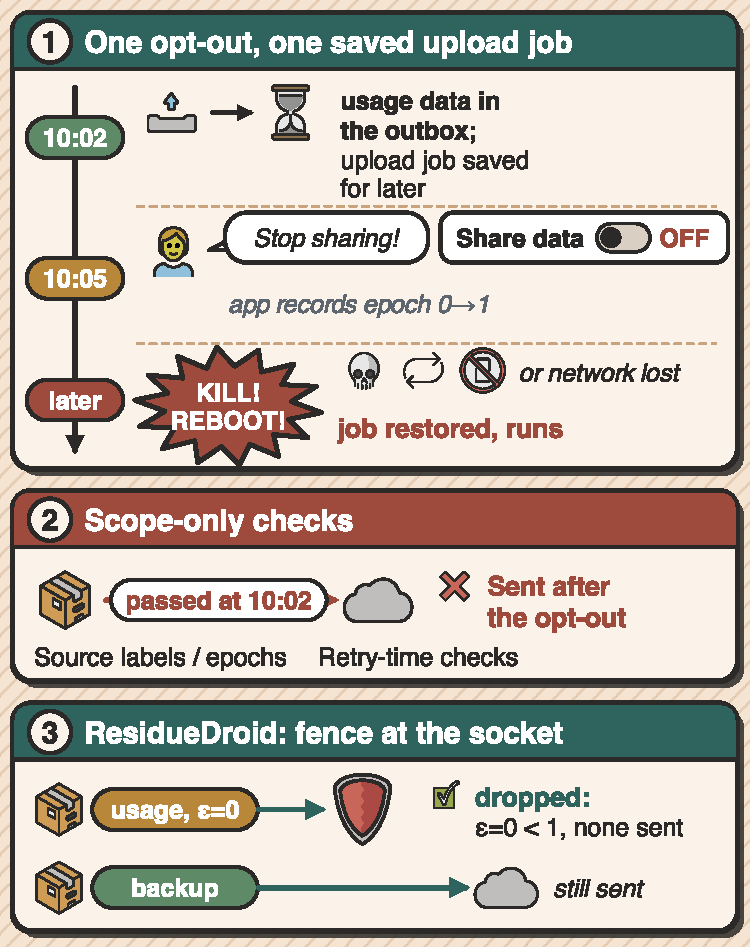
\includegraphics[width=\columnwidth]{figures/fig1.pdf}
\caption{(1)~A saved upload job outlives an opt-out across a kill, a reboot or a network loss. (2)~Checks made before submission let the data through. (3)~With \sys the label travels with the data and the fence at the socket drops it, while permitted flows such as backup still go out. Panel 2 names the information and retry checks needed by the fixture; it reports no population failure rate. Bytes already accepted before the opt-out are not recalled. Icons: OpenMoji (CC BY-SA 4.0).}
\Description{Comic with a vertical timeline panel and two stacked outcome panels. At 10:02 usage events and a summary go into an outbox and an upload job is saved; at 10:05 the user turns the Share data toggle off; later the process is killed, the device reboots or the network drops and the job is restored. With checks made earlier the data is sent after the opt-out. With ResidueDroid the labelled usage data is dropped at a fence at the socket while a backup flow is still sent.}
\label{fig:overview}
\end{figure}


Mobile apps rarely send data the moment they collect it. Usage events, crash reports, location history and derived
summaries go into a local outbox. A deferred job uploads them later, when the device has connectivity, is charging, or the
batch is large enough. Android makes this deferral durable on purpose. \texttt{JobScheduler} restores persisted jobs after
reboot, WorkManager keeps its own database of pending work~\cite{android_jobscheduler,android_workmanager}, and analytics SDKs
flush their outboxes when the app starts. Durability is what makes background uploads reliable. It also means that the upload
path can outlive the user's decision to stop it.

Consider an app whose settings say ``Share usage data''. It has queued twelve events and a summary derived from them when the user
switches the toggle off (Figure~\ref{fig:overview}). The app does the usual things. It stops collecting, it may cancel the
upload job, and its job checks the toggle before it starts. But the summary was copied into a job filed under
``diagnostics''. The process is killed and the job is restored by the system. Or the network drops after the job has started
and its retry loop resends the batch it already prepared. In each case data that the app promised to stop sending leaves the
device after the promise was made. The integration lacks a check that remains effective until socket handoff.

This paper is about that gap, and it is deliberately narrow. Withdrawal inconsistency itself is not new.
MowChecker~\cite{du2024mowchecker} statically finds withdrawal choices that do not control third-party collection.
CleanOS~\cite{tang2012cleanos}, Pebbles~\cite{spahn2014pebbles} and Weir~\cite{nadkarni2016weir} established data management
and information-flow enforcement on Android. Taint tracking~\cite{enck2010taintdroid,arzt2014flowdroid} finds flows to the
network. Two problems remain. The first is \emph{deferred} egress: data collected before an explicit withdrawal reaches the
network afterwards through persisted work, across process death, reboot and connectivity changes. The second is where a
cooperative app must enforce its own contract so that no lifecycle interleaving defeats it. We also refuse two simplifications.
First, a stored residue is not a violation. An OS permission revocation, an in-app opt-out, a processing restriction and a
deletion request are different contracts (\S\ref{sec:contracts}), and we judge each workload against the one it states.
Second, bytes already handed to the network cannot be recalled. A device-side mechanism can only control what it
\emph{newly} commits.

\paragraph{Approach.} \sys combines three small mechanisms. Durable per-scope \emph{epochs} turn a withdrawal into a
transaction. \emph{Persistent job lineage} stores a label of source scopes and epochs in the same row, or the same
persisted job input, as every copy of the data, including derived data. A \emph{late egress fence} evaluates the app's stated
contract before each bounded nonblocking socket write, inside a critical section shared with withdrawal. Under complete
mediation, durable labels and this serialization, no newly accepted supported prefix carries a source that the current policy invalidates (Theorem~\ref{thm:sound}). An earlier check without effective later cancellation admits a violating interleaving when withdrawal invalidates the source; its
probability follows from the job's commit timing (Theorem~\ref{thm:race}).

\paragraph{Evidence.} The evaluation separates information requirements from final placement.
The \corpusN-app static screen identifies candidate deferred paths, without inferring violations (\S\ref{sec:measure}).
The ten-tenant fixture exposes source-lineage loss in derived summaries (T1), stale epochs after re-grant (T5), and unchecked retry paths (T8).
These are mechanism-specific counterexamples whose frequencies depend on the selected workload mix (\S\ref{sec:eval}).
When layered early checks receive the same durable metadata, they have no confirmed violations in the measured lifecycle schedules; the fence's additional benefit is confined to a residual check-to-write interleaving, demonstrated separately with a controlled HTTPS buffering barrier.
The ACRA preference-only embedding uploads a queued report in \acraStockLeak{} trials after the harness disables reporting. It has no user-facing promise to delete that queue, so this observation alone is not a contract violation. A separate setting explicitly invalidates queued reports and exercises the fenced integration (\S\ref{sec:eval-acra}).

\paragraph{Contributions.}
(1) A contract-separated formulation of deferred egress after withdrawal, with an oracle that judges each submission
against the stated contract at an explicitly stated observation boundary. (2) \sys's persistent job lineage and serialized late fence, with a
soundness theorem for supported paths, a race theorem for earlier check points, and information requirements for lineage and
epochs. (3) A static measurement of an F-Droid corpus, a real-library case study, and a controlled emulator evaluation with
permitted-flow controls, matched transports and explicit uncovered paths. The artifact includes sources, raw logs, exclusions and deterministic generators.

\section{Withdrawal Contracts and Deferred Work}
\label{sec:background}

\subsection{Four contracts, not one}
\label{sec:contracts}

``The user said stop'' covers several different promises. We separate four, following the distinctions that consent
studies~\cite{nguyen2021sharefirst,nguyen2022freely,kollnig2021faitaccompli} and data-deletion work~\cite{reardon2013deletion,garg2020deletion,shastri2020gdprbench}
already draw, and evaluate every fixture against the contract it states (Table~\ref{tab:contracts}).

\begin{table}[t]
\centering
\caption{Withdrawal contracts. ``Pending'' says whether data collected \emph{before} the withdrawal is covered.}
\label{tab:contracts}
\mtab
\begin{tabular}{@{}>{\raggedright\arraybackslash}p{2.2cm}>{\raggedright\arraybackslash}p{1.6cm}>{\raggedright\arraybackslash}p{1.15cm}>{\raggedright\arraybackslash}p{2.8cm}@{}}
\toprule
\mhead Contract & Purposes revoked & Pending & Violation evidence \\
\midrule
OS permission revocation & none (new access only) & no & none from prior data; residue is \emph{not} a violation \\
In-app opt-out (stop collecting) & all & stated & new collection; prior data only if the app says ``discard'' \\
Processing restriction & named purpose & yes & use for that purpose; other purposes stay legal \\
Deletion request & all & yes & any later egress of the data or its derivatives \\
\bottomrule
\end{tabular}
\end{table}

An \emph{OS permission revocation} (\texttt{pm revoke}, or the settings toggle) only stops future access to a source.
Android kills the process, but nothing in the platform contract obliges the app to forget what it already read,
so a later upload of earlier location fixes is residue, not a violation~\cite{felt2011demystified,wang2022aper}.
An \emph{in-app opt-out} is the app's own promise. Some wordings stop collection only (``we will stop collecting''); others
also discard what is queued (``we will no longer send usage data''). A \emph{processing restriction} withdraws one purpose,
such as personalisation, while storage and backup stay permitted. A \emph{deletion request} covers the data and anything derived
from it. Throughout, a submission is a \emph{prohibited submission} only if its contents contradict the contract the app states, at the time
the bytes leave the device. Stored residue alone never counts. We make no legal claims.

\subsection{Deferred work survives the withdrawal}
\label{sec:deferred}

Persisted \texttt{JobScheduler} jobs are written to
the system's job store and restored after reboot~\cite{android_jobscheduler}. WorkManager keeps its own SQLite database and reschedules work
after app restarts and reboots~\cite{android_workmanager}. Alarms do not survive reboot, so apps re-arm them from their own state. SyncAdapters
run on the system's schedule. Analytics and crash-reporting SDKs add another layer: they keep an outbox, and many flush it when the app
starts.

On the Android~13 image we use (\S\ref{sec:setup}), we observed the following lifecycle facts directly over \lcTrials{} campaign trials
(Table~\ref{tab:lifecycle}). Each one shapes which enforcement points can see a queued upload.
\begin{table}[t]
\centering
\caption{Measured lifecycle behavior of a persisted upload job (\vname{none}, AVD~A). Counts of trials; ``by-value job'' is T2's summary job, whose data exists only in its extras.}
\label{tab:lifecycle}
\mtab
\begin{tabular}{@{}lrrrrr@{}}
\toprule
\mhead Schedule & trials & job ran & re-enqueued & by-value job ran & median s \\
\midrule
\textsf{pen} & 50 & 50 & 0 & 50 & 43 \\
\textsf{kill} & 50 & 50 & 0 & 50 & 43 \\
\textsf{fstop} & 50 & 0 & 50 & 0 & 19 \\
\textsf{reb} & 50 & 50 & 0 & 50 & 51 \\
\textsf{rev} & 50 & 50 & 0 & 50 & 24 \\
\bottomrule
\end{tabular}
\end{table}

\begin{itemize}[leftmargin=*,nosep]
\item \textbf{Reboot.} Persisted jobs are restored and run after boot. A check made at enqueue time is therefore arbitrarily old when the job runs.
\item \textbf{Process death} (\texttt{kill -9}, or a runtime-permission revocation, which kills the app). Jobs stay scheduled, and JobScheduler restarts the process to run them.
\item \textbf{Force-stop} removes the app's scheduled jobs. When the user next opens the app, an outbox-driven startup path re-enqueues the work. A job whose \emph{only} copy of the data was in its extras is lost.
\item \textbf{Network loss mid-job.} An upload loop retries the batch it already prepared. A check made at job start ran before the withdrawal.
\end{itemize}
Withdrawal is a user action at an arbitrary time, so it can land in any of these windows. Our question is which enforcement point
still sees it.

\section{How Common Are Deferred Egress Paths?}
\label{sec:measure}

Before building a mechanism, we asked how often apps combine the three ingredients of the problem: persisted deferred
work, a network sink reachable from a deferred-job entry point, and a user-facing telemetry or consent control. This is a
\emph{candidate} screen. Static analysis cannot see runtime state or app wording, so it cannot establish a violation.

\paragraph{Corpus.} From the F-Droid index~\cite{fdroid} (fetched 2026-11-08, SHA-256 recorded), we took the latest version
of every app that requests \texttt{INTERNET} and is at most 80\,MB, giving \eligibleN{} apps. We selected all \trackN{} that
carry F-Droid's \emph{Tracking} anti-feature, plus a seeded random sample of \randN{} others. All \corpusN{} APKs were
downloaded from \texttt{f-droid.org} and verified against the index hashes. F-Droid apps are open source and often minified,
so library method names may be renamed. We therefore detect WorkManager through \texttt{ListenableWorker} subclasses,
whose names are kept for reflection, as well as through API references.

\paragraph{Analysis.} Our scanner (\S\ref{sec:impl}) finds deferred-job entry points: \texttt{doWork}/\texttt{startWork} of
WorkManager workers, \texttt{onStartJob} of \texttt{JobService}s, and \texttt{onPerformSync}. From each, it searches
breadth-first for a network sink (\texttt{HttpURLConnection}, OkHttp, Retrofit, Volley, Ktor, raw sockets and similar). The
search is over-approximate. We validated it on a seeded sample of \valN{} app-code entries in apps with a consent signal,
judging from class names and app purpose whether network use is on the job's own path. Of \valShallowN{} entries within three hops, \valShallowYes{} were judged plausible and \valShallowUnclear{} unclear;
of \valDeepN{} deeper entries, \valDeepYes{} were plausible, \valDeepUnclear{} unclear and \valDeepNo{} implausible. These class-name/app-purpose
judgments do not validate runtime paths or estimate false negatives. We report two screening thresholds
(three hops and any depth), not lower and upper bounds on real flows. Consent signals are identifier-like constants pairing a topic token
(\textit{analytics}, \textit{telemetry}, \textit{crash}, \textit{consent}, ...) with a control token (\textit{enable},
\textit{opt}, \textit{send}, ...), or English toggle-like resource strings such as ``Share anonymous usage statistics''.

\begin{table}[t]
\centering
\caption{F-Droid corpus screen: apps (\%). Random-stratum percentages carry Wilson 95\% intervals conditional on the screen. Tracking is a census of eligible tracking apps. $^\dagger$persisted deferred work + entry$\to$network + consent signal.}
\label{tab:corpus}
\mtab
\begin{tabular}{@{}lrr@{}}
\toprule
\mhead Feature & Tracking ($n{=}$60) & Random ($n{=}$300) \\
\midrule
Network API & 57 (95) & 277 (92) [89, 95] \\
\texttt{JobScheduler} & 32 (53) & 183 (61) [55, 66] \\
\quad \texttt{setPersisted} & 22 (37) & 114 (38) [33, 44] \\
WorkManager & 9 (15) & 45 (15) [11, 19] \\
AlarmManager & 37 (62) & 188 (63) [57, 68] \\
SyncAdapter & 0 (0) & 3 (1) [0, 3] \\
Persisted deferred work (any) & 22 (37) & 116 (39) [33, 44] \\
Entry $\to$ network, $\le$3 hops & 5 (8) & 17 (6) [4, 9] \\
Entry $\to$ network, any depth & 13 (22) & 53 (18) [14, 22] \\
Persisted + entry$\to$net, $\le$3 & 4 (7) & 17 (6) [4, 9] \\
Persisted + entry$\to$net, any & 10 (17) & 50 (17) [13, 21] \\
Consent/telemetry signal & 23 (38) & 42 (14) [11, 18] \\
Candidate, $\le$3 hops$^\dagger$ & 3 (5) & 5 (2) [1, 4] \\
Candidate, any depth$^\dagger$ & 6 (10) & 12 (4) [2, 7] \\
Telemetry/crash SDK & 19 (32) & 14 (5) [3, 8] \\
Native libraries & 38 (63) & 210 (70) [65, 75] \\
\bottomrule
\end{tabular}
\end{table}


\paragraph{Findings.} Table~\ref{tab:corpus} reports each sampling stratum separately: the tracking stratum is a census
within the eligible index, random-stratum intervals are conditional on classification, and we do not pool the
oversampled strata. With only \valN{} validation judgments, the plausible fraction is \valYes{}/\valN{} (Wilson 95\%
interval from \valYesLo{}\% to \valYesHi{}\%), and \valUnclear{} remain unclear. Summed over both strata (a count of
apps, not a pooled rate), between \candConsentLoN{} (three-hop screen) and \candConsentHiN{} (any depth) screened apps persist deferred work, reach the network from a deferred-job entry
point and carry a consent or telemetry signal; neither count estimates a contract-violation prevalence. Only
\pctPollStop{}\% of app-code workers poll \texttt{isStopped()}, which does not show whether cancellation interrupts
uploads; between-batch stopping is a fixture assumption, not a corpus finding. Native code, which most screened apps in
both strata ship, is a path no Java-level fence mediates.

\paragraph{Stated promises.} A consent signal does not say what an app promises. We coded the user-facing wording of
all \promiseApps{} apps with a consent signal (\promiseCand{} of them candidates), using the toggle-like strings in each APK
and its F-Droid listing; privacy policies were not collected. A language model applied written rules to every app and
flagged \promiseFlagged{} for review; an author re-read those and recoded \promiseRecoded{}. In this sample,
\promisePending{} apps word a switch as sending or sharing data (\promiseCandPending{} of the candidates), which we read as
also covering queued data; \promiseCollectOnly{} word it as collection only; \promisePrompt{} only offer to send an
individual report; \promiseUnclear{} expose only code identifiers or unclear wording; \promiseFalse{} are scanner false
positives. \promiseDelete{} offer deletion and \promiseRestrict{} a purpose restriction. Only the first group makes
queued egress after withdrawal a contract violation. These counts describe the surveyed apps, not F-Droid.

ACRA appears in \acraApps{} apps, but its preference keys are library constants and do not show an exposed toggle
(\S\ref{sec:eval-acra}). The screen shows that the ingredients co-occur in the screened apps, not how often they combine into a violation;
the rest of the paper turns to controlled, contract-aware experiments.

\section{ResidueDroid Design}
\label{sec:design}

\subsection{Scope and threat model}
\label{sec:scope}

\sys is a \emph{cooperative} mechanism. The developer, or an SDK vendor, wants the app to keep its stated contract and links
\sys to do so. We do not defend against a malicious app, which can always exfiltrate data through a path we do not
mediate~\cite{reardon2019fiftyways}. The adversary is the schedule: a withdrawal arrives at an arbitrary time relative to queued
work, process death, reboot, force-stop and connectivity changes. A \emph{supported path} is a flow whose data is stored through
\sys's labelled stores and whose network submission goes through \sys's egress wrapper. Everything else is \emph{uncovered}.
That includes native code (JNI), custom network stacks such as raw sockets or embedded HTTP clients that bypass the wrapper,
WebViews, IPC to other apps, and any flow the developer did not route through the wrapper. We claim nothing for uncovered
paths. The raw-socket tenant measures one directly in \S\ref{sec:eval}.

\sys also cannot recall bytes. Data handed to the network before the withdrawal takes effect may still arrive afterwards, and
server-side copies are outside the device. The guarantee orders each accepted socket prefix relative to policy updates. A write can accept
only part of a request; its authorization log, local acceptance and remote receipt are distinct.

\subsection{Three mechanisms}
\begin{figure}[t]
\centering
\begin{tikzpicture}[font=\scriptsize,
  st/.style={draw=mSlate,rounded corners=2pt,fill=mNavy!7,align=center,inner sep=2.5pt,minimum height=0.7cm},
  op/.style={draw=mSlate,rounded corners=2pt,fill=mOchre!16,align=center,inner sep=2.5pt,minimum height=0.7cm},
  fe/.style={draw=mTeal,thick,rounded corners=2pt,fill=mTeal!11,align=center,inner sep=2.5pt,minimum height=0.85cm},
  arr/.style={-{Latex[length=1.5mm]},thick,draw=mInk!85}]
\node[op,text width=1.15cm] (col) at (0,0) {collect\\$\ell{=}\{(s,\epsilon)\}$};
\node[st,text width=1.3cm] (rows) at (1.8,0.5) {outbox rows\\+ label};
\node[st,text width=1.3cm] (der) at (1.8,-0.5) {derived rows\\$\ell{=}\bigcup$ inputs};
\node[st,text width=1.25cm] (job) at (3.55,0) {persisted job\\extras + label};
\node[fe,text width=1.2cm] (fence) at (5.55,0) {\icon[0.9em]{shield} fence\\check each\\chunk};
\node[draw=mSlate!70,rounded corners=2pt,fill=mSlate!8,align=center,text width=0.7cm,minimum height=0.7cm] (net) at (7.0,0) {\icon{cloud}\\socket};
\node[op,text width=1.55cm] (wd) at (3.55,-1.35) {withdraw (txn):\\$\epsilon{+}{+}$, $a{=}0$};
\node[st,text width=1.15cm] (gr) at (5.55,-1.35) {grants $\epsilon,a$\\(durable)};
\draw[arr] (col) -- (rows); \draw[arr] (col) -- (der); \draw[arr] (rows.east) -- (job); \draw[arr] (der.east) -- (job);
\draw[arr] (job) -- (fence);
\node[font=\tiny,align=center] at (4.3,0.72) {restored after kill / reboot};
\draw[arr] (fence) -- (net);
\draw[arr] (wd) -- (gr); \draw[arr,dashed] (gr) -- node[right,font=\tiny]{read} (fence);
\draw[thick,mTeal,dotted] (wd.north east) -- node[above left=-1pt,font=\tiny,text=mTeal]{lock $L$} (fence.south west);
\end{tikzpicture}
\caption{\sys data path. Labels travel with every persisted copy. The fence reads durable epochs and writes each bounded chunk while holding the lock that withdrawals also take.}
\Description{Source labels are stored with outbox rows, combined for derived rows and copied into persisted job extras. A fence checks each outgoing chunk against durable grants while sharing a lock with withdrawal.}\label{fig:design}
\end{figure}

Figure~\ref{fig:design} shows how the three mechanisms fit together.


\paragraph{Durable epochs.} For every withdrawable scope $s$, such as \textit{analytics} or \textit{profile}, \sys keeps a
durable epoch $\epsilon(s)$ and a flag $a(s)$. A withdrawal runs as one transaction that increments $\epsilon(s)$, clears
$a(s)$ and, for a deletion request, deletes local rows. A re-grant sets $a(s)$ again but keeps the epoch. Data collected
afterwards belongs to the new epoch, and data from older epochs stays invalid. The state lives in the app's SQLite database, so
it survives process death and reboot.

\paragraph{Persistent job lineage.} Each persisted datum carries a label $\ell(d)\subseteq\{(s,\epsilon)\}$, the scopes and
epochs of the sources it was computed from. The label is written \emph{in the same row or the same job input} as the data,
so it is committed atomically with the data. Collection assigns $\{(s,\epsilon(s))\}$, and derivation takes the union of its
inputs' labels. When data is copied into a job's persisted input (a \texttt{PersistableBundle} or WorkManager \texttt{Data}),
the label is copied with it. The label therefore survives in the job store, which a database deletion does not reach.

\paragraph{Late, serialized egress fence.} Every supported submission passes through
\texttt{Fence.submit(purpose, items)}. The audited HTTP adapter connects outside the lock,
encodes the request with a conservative union of its source labels, and writes chunks of at most
4\,KiB. Before each nonblocking write it acquires the same lock as withdrawal and rechecks
those labels. A zero-byte return is no handoff; a positive return records exactly the accepted
prefix. Waiting for socket readiness and reading the response occur outside the lock.
If policy changes after a partial send, the adapter closes the connection and suppresses the
remainder; previously accepted bytes remain outstanding. The contract rule for an item with label
$(s,e)$ and purpose $p$ is
\begin{equation}
\begin{aligned}
\mathit{forbid}(s,e,p)\;=\;{}&p\in R_s\;\wedge\;\big[(\pi_s\wedge e<\epsilon(s))\\
&\vee\;(e=\epsilon(s)\wedge\neg a(s))\big],
\end{aligned}
\label{eq:rule}
\end{equation}
where $R_s$ is the set of purposes the contract revokes and $\pi_s$ says whether it covers pending data
(Table~\ref{tab:contracts}). An item is forbidden if any element of its label is forbidden. For an OS-permission tenant
$R_s=\emptyset$, so prior data is never blocked. For a processing restriction, $R_s=\{\textit{personalisation}\}$, so backup
continues. For a ``stop collecting'' opt-out, $\pi_s$ is false, so queued data may still flush.

\begin{algorithm}[t]
\caption{Audited HTTP fence, with source labels on every retry}
\label{alg:fence}
\begin{algorithmic}[1]
\Require purpose $p$, encoded bytes $B$, durable source union $\ell$
\State Connect outside $L$; set operation deadline
\While{unsent bytes remain}
\State Wait for socket readiness outside $L$
\State Acquire $L$ within deadline
\State Read durable policy; reject unknown or forbidden labels
\State Attempt nonblocking write of at most 4\,KiB
\State Record returned accepted count; release $L$
\EndWhile
\State Read response outside $L$; retain source labels on retry
\end{algorithmic}
\end{algorithm}

\paragraph{Why this placement.} An early check can leave a window when an applicable withdrawal precedes an unprotected send.
Cancellation can miss re-enqueued or running work if it does not reach the transport. A check at enqueue misses a job queued before the withdrawal. A check at
job start misses everything the job prepared before the withdrawal and submits after it, including retries. Our declared-scope egress baseline misses a derived source when that source is invalidated
but the declared scope still passes. A boolean
consent flag without epochs lets old data through after a re-grant. \S\ref{sec:theory} turns each gap into a statement, and
\S\ref{sec:eval} measures each one.

\paragraph{Cost and composition.} One app-wide coordinator combines a local mutex with an
exclusive file lock. This simple design can briefly delay unrelated scopes, and storage or
scheduling delays can exceed nominal deadlines. Five-second operation deadlines are best-effort
failure bounds, not real-time guarantees. A failed or pending withdrawal is never acknowledged
as successful. Layered cancellation and early checks can reduce wasted work; the stated prefix-level guarantee uses a check for each final chunk. The old whole-request HTTP-stream wrapper is retained as a stream-wrapper
comparison, not used to justify the channel handoff boundary.

\section{What the Fence Guarantees}
\label{sec:theory}

The durable state $\sigma$ contains scope epochs, grant flags and labelled copies.
Table~\ref{tab:lifecycle-states} lists the states of one submission. An authorization
log is an observation of intent, not a send. A \emph{handoff} $c$ is acceptance of a
positive byte prefix by the audited socket transport; a write may accept fewer bytes
than requested or none. The guarantee concerns each accepted prefix, including a
prefix of a request that never completes.

\begin{table}[t]\centering
\caption{Lifecycle of one submission, with the artifact's event names. The fence check shares the withdrawal lock (A3); earlier checks do not.}
\label{tab:lifecycle-states}\mtab
\begin{tabular}{@{}p{0.40\columnwidth}p{0.18\columnwidth}p{0.34\columnwidth}@{}}\toprule
\mhead State (event) & Check & Crash or loss here\\\midrule
Labelled copy stored (\texttt{COLLECT}) & none & label survives with the row (A2)\\
Job queued, label in row or extras (\texttt{ENQUEUE}) & enqueue check & job restored after reboot with its epochs\\
Batch prepared (\texttt{JOBSTART}, \texttt{AUTHORIZATION\_LOGGED}) & job-start check & nothing accepted; retry rereads policy\\
TLS record buffered (\texttt{TLS\_BUFFERED}) & none & nothing accepted\\
Prefix handed off (\texttt{WRITE\_ATTEMPT}, \texttt{BYTES\_ACCEPTED}) & fence, per write & count may be unlogged: unknown, never zero\\
Request received (receiver log) & none & accepted bytes may still arrive (Prop.~\ref{prop:recall})\\
Response received (\texttt{RESPONSE\_RECEIVED}) & none & lost response: retry may duplicate\\
\bottomrule\end{tabular}\end{table}

\begin{assumption}[Supported path]\label{as:sp}
(A1) Every supported byte is sent through Algorithm~\ref{alg:fence}, with one writer
per socket and no unmediated asynchronous sender below its check. For TLS, the checked bytes are application-record ciphertext: the request's conservative source union remains attached to every encrypted record and partial-record remainder. Encryption may precede checking; each subsequent socket write must recheck policy. Handshake traffic contains no request data. TLS early data, renegotiation and external writers are excluded.
(A2) Every persisted copy carries atomically stored, over-approximate source labels;
missing or invalid labels fail closed. Labels on retries retain the collection epochs.
(A3) Each bounded, nonblocking write and its policy check share a process/cross-process
lock with withdrawal and re-grant. A withdrawal commits its policy transaction before
acknowledgement. Policy state survives process failure; an unreadable store fails closed.
The model assumes working durable storage, not recovery from arbitrary power loss.
\end{assumption}

\begin{theorem}[Soundness of accepted prefixes]\label{thm:sound}
Under A1, A2 and A3, every source label of a supported prefix accepted at $c$ satisfies
$\neg\mathit{forbid}_{\sigma(c)}(s,e,p)$. Thus no prefix accepted after an acknowledged
withdrawal carries a source that remains invalid under the stated contract.
\end{theorem}
\begin{proof}
Consider one write and its preceding check in the same critical section. A3 excludes
policy changes between the check and every byte acceptance during that write. A2
includes every source in the checked label union, and the check rejects any forbidden
source. Hence every accepted prefix satisfies the rule. Crashes add no exception
(Table~\ref{tab:lifecycle-states}): a prefix accepted by an interrupted write is still
covered by its check, even if no count is logged, and after restart the next attempt
reacquires the lock and rereads durable policy, so it cannot reuse an earlier authorization.
\end{proof}

Exact labels avoid policy-induced false positives only when labels and policy are
available and valid. Over-approximation, fail-closed migration, timeouts and network
failure can still prevent permitted delivery. Soundness is not an availability claim.

\begin{theorem}[Race for earlier checks]\label{thm:race}
Suppose a check $q$ admits a source that a later withdrawal would invalidate for the
submission's purpose, and the path can still hand off that source at $c>q$ without
another effective check or cancellation. Then a withdrawal in $(q,c)$ yields a forbidden
handoff. If a single such withdrawal $W$ is independent of fixed handoff offsets
$c_1<\cdots<c_k$, all carrying sources invalidated by $W$, with no intervening re-grant and $n_i>0$ newly handed-off source items,
\begin{equation}
\begin{aligned}
\Pr[\text{violation}]&=\Pr[q<W<c_k],\\
\mathbb E[\#\text{forbidden item handoffs}]&=\sum_i n_i\Pr[q<W<c_i].
\end{aligned}\label{eq:race}
\end{equation}
These equations concern that schedule model; cancellations or retries that depend on
$W$ require a different model.
\end{theorem}
\begin{proof}
Place the applicable withdrawal between the passing check and the unprotected write.
The path still sends, by hypothesis. Summing the corresponding indicator variables
gives the expectation; the last interval contains the earlier intervals.
\end{proof}

\begin{proposition}[Information needed by the check]\label{prop:nec}
A declared-scope check can admit an invalid source when a withdrawal invalidates the
actual source scope while the declared scope still passes. A current boolean alone
cannot distinguish old and new data after withdrawal and re-grant when the contract
invalidates pending old data. Source lineage and retained epochs supply these distinctions;
equivalent representations are possible.
\end{proposition}

\begin{proposition}[No recall]\label{prop:recall}
A prefix accepted before withdrawal may arrive after acknowledgement. A device-side
fence cannot guarantee recall of bytes already accepted by the transport.
\end{proposition}

Each retry is checked afresh, but the mechanism provides neither server-side deletion nor
exactly-once delivery. The stream-wrapper evaluation's pre-write sequence markers cannot establish which
prefixes were outstanding; the channel wrapper records acceptance and receipt separately.

\section{Implementation}
\label{sec:impl}

\paragraph{Library and integration.} The implementation uses a shared Java
\texttt{SocketChannel}~\cite{android_socketchannel} HTTP/1.1 sender and a TLS~1.2 adapter built on \texttt{SSLEngine}~\cite{java_sslengine}. The latter verifies the peer certificate and host, encrypts at most 4\,KiB of plaintext per wrap, and rechecks policy before each at-most-4\,KiB ciphertext write. Proxies, redirects, pooled writers, early data and renegotiation are excluded. Its positive write return is socket acceptance, not server delivery. A local
mutex plus file lock coordinates threads and processes. The ACRA and Matomo embeddings and their sizes are in
Appendix~\ref{app:sdk}.

\paragraph{Fixture app (\lab).} To compare enforcement points on identical schedules, we built a fixture app with ten
\emph{tenants}. Each is an independent workload with its own scope, stated contract and persisted jobs (Table~\ref{tab:tenants}).
Every tenant collects 12 records tagged with synthetic tracer strings such as \texttt{RD-pen007-T1-e0-03} into a SQLite
outbox. Tenants with a summary also derive one daily summary row whose content lists its source tags, and copy it into a
persisted summary job. All uploads use persisted \texttt{JobScheduler} jobs with a network constraint, in batches of four
records with up to five in-job attempts and exponential backoff. They stop cooperatively between batches on
\texttt{onStopJob}. The app's startup path re-enqueues an upload whenever its outbox holds unsent rows and no job is
scheduled, as analytics SDKs commonly do. One package is installed per enforcement variant, all from the same code:
\begin{itemize}[leftmargin=*,nosep]
\item \vname{none}: stops collection only.
\item \vname{cancel}: additionally cancels the withdrawn scope's jobs and purges its unsent outbox.
\item \vname{enqueue}: checks consent at every enqueue, including the startup path.
\item \vname{jobstart}: checks consent at job start.
\item \vname{conv}: cancel + enqueue + job-start checks, the strongest conventional combination.
\item \vname{egress}: a serialized egress check on the job's declared scope, without lineage or epochs.
\item \vname{rd}: \sys.
\end{itemize}
Two ablations change one \sys mechanism each. \vname{volatile} keeps labels in memory and fails open on unknown
provenance. \vname{taint} uses durable lineage but a contract-unaware rule, so any withdrawal or revocation of a source
blocks all its uses, as a deliberately over-broad synthetic policy would. It is not an implementation of TaintDroid or a comparison with a complete taint system. A tenth package, \vname{noser}, drops serialization and is
used only in the race micro-benchmark.

Five matched variants share durable lineage, epochs, and the same chunk transport:
\vname{menqueue}, \vname{mstart}, \vname{mlayer} (cancellation plus enqueue, job-start and retry checks),
\vname{mfence}, and \vname{mboth} (layered checks plus final fencing). All retain source labels
in copied job inputs. Their comparisons isolate final placement more closely than the boolean-only baselines.

\paragraph{Harness and oracle.} A host sink, reached via \texttt{10.0.2.2}, logs every request and waits 300\,ms before
responding, emulating a wide-area server. The oracle (\S\ref{sec:setup}) is a separate Python reimplementation of the
contract table. It never reads the app's labels or decisions, but takes order from device-logged events; the receiver is
the only outside observer. The split policy for mixed requests, the real-app embedding,
and the phone and throttled-link harnesses are described in Appendix~\ref{app:round3impl}.

\paragraph{Static scanner.} For the measurement (\S\ref{sec:measure}) we wrote a standard-library-only DEX parser. It
reads string, type, method and class tables, decodes Dalvik code items, and builds an over-approximate call graph:
class-hierarchy resolution below app-defined types, and allocation edges to callback methods of allocated classes.

\section{Evaluation}
\label{sec:eval}
\subsection{Setup}
\label{sec:setup}

\paragraph{Platform.} Lifecycle and SDK runs use the stock Android~13 emulator image
(android-33 google\_apis arm64-v8a rev.~17, build TE1A.240213.009), emulator 37.2.13, on an 18-core Apple-silicon host. The stream-wrapper campaign uses two AVDs side by side; the enlarged matched campaign uses four read-only instances of each of those two configurations. HTTP/TLS cost and label-error tests use a separate Android~15 emulator on the same host; exact fingerprints and host load are archived.
AVD~A runs \vname{none}, \vname{cancel}, \vname{enqueue}, \vname{jobstart}, \vname{conv} and \vname{rd}. AVD~B runs
\vname{egress}, \vname{rd}, \vname{volatile} and \vname{taint}. Repeating \vname{rd} on both AVDs does not remove variant--AVD confounding: cross-AVD comparisons are descriptive. Matched channel variants run within each AVD. Before every trial each package is cleared with \texttt{pm clear}, granted location, opened once,
and placed in the \texttt{active} standby bucket. Without that last step JobScheduler never ran our jobs: a never-opened app
sits in the \texttt{NEVER} bucket.

\begin{table}[t]
\centering
\caption{\lab tenants. Every tenant has 12 tagged records; ``sum.'' tenants also derive a summary (declared scope in brackets).}
\label{tab:tenants}
\mtab\setlength{\tabcolsep}{2.5pt}
\begin{tabular}{@{}l>{\raggedright\arraybackslash}p{1.85cm}>{\raggedright\arraybackslash}p{1.75cm}>{\raggedright\arraybackslash}p{2.9cm}@{}}
\toprule
\mhead Tenant & Contract & Withdrawal & What it tests \\
\midrule
T1 & opt-out, discard & in-app & summary filed as \textit{diagnostics} (lineage) \\
T8 & opt-out, discard & in-app & same, summary correctly declared \\
T2 & deletion request & in-app + delete rows & summary copy in job extras \\
T5 & opt-out, discard & withdraw, re-grant & epoch vs.\ boolean (+4 new records) \\
T9 & opt-out, discard & in-app & raw-socket upload (uncovered path) \\
T10 & opt-out, discard & in-app & encrypted body (unattributable) \\
\midrule
T3 & opt-out, flush allowed & in-app & FP control: queued data may go \\
T4 & restriction & personalisation & FP control: backup must go \\
T6 & none & none & FP control: everything must go \\
T7 & OS permission & \texttt{pm revoke} (in \textsf{rev}) & FP control: prior fixes may sync \\
\bottomrule
\end{tabular}
\end{table}

\paragraph{Schedules.} Each trial sets up all ten tenants in every package, injects one schedule, waits until no job of
ours remains registered (polling \texttt{dumpsys jobscheduler}), and then reads each app's event log with \texttt{sqlite3}
as root, which does not start the app. The seven schedules are:
\begin{itemize}[leftmargin=*,nosep]
\item \textsf{pen}: withdraw while the jobs are pending.
\item \textsf{kill}: withdraw, then \texttt{kill -9}.
\item \textsf{fstop}: withdraw, force-stop, reopen the app 3\,s later.
\item \textsf{reb}: withdraw, then reboot.
\item \textsf{rev}: withdraw, then \texttt{pm revoke} location, which kills the app.
\item \textsf{net}: connectivity cut as the jobs start and restored 6\,s later; withdrawal 1.5--1.8\,s after job start.
\item \textsf{infl}: withdrawal at a seeded uniform offset in $[0,1.6]$\,s after the upload job starts.
\end{itemize}
In \textsf{net} and \textsf{infl}, jobs are started with \texttt{cmd jobscheduler run -f}, and the withdrawal is injected
inside the app relative to the job's own start, so its timing is precise. In \textsf{net}, each app gets its own 6\,s outage in
turn, during which only the trigger uploads of T8, T2, T5 and T4 are started. The outage is a guest firewall rule rejecting traffic to the
server. We first tried \texttt{svc wifi/data disable}, but it did not cut the apps' traffic reliably, and starting all apps' jobs
at once let JobScheduler's concurrency limit decide which variant saw the outage. The configuration trials using those two methods are excluded. Schedule parameters are derived from a seed per
(schedule, trial), so both AVDs replay identical schedules.

\paragraph{Oracle and metrics.} Ground truth comes from the sink. Tags are visible in plaintext payloads, and a summary's
content lists its source tags. The stream-wrapper device sequence orders withdrawals and pre-write authorization logs,
not actual byte acceptance. Baselines can therefore undercount forbidden handoffs in the
log-to-write gap. Missing sequence evidence is ambiguous; host receipt time alone cannot
reconstruct a socket-handoff order. We preserve the authorization-order estimand explicitly.
The channel oracle uses paired write-attempt/accepted-count events and the withdrawal
transaction order; interrupted or overlapping observations remain unknown. We report:
\begin{itemize}[leftmargin=*,nosep]
\item \emph{Violation rate}: the fraction of tenant-trials with at least one prohibited item, with trial-cluster uncertainty, keeping all tenants and paired variants together.
\item \emph{Prohibited items} per tenant-trial.
\item \emph{Legit deficit}: permitted items that a variant had not delivered when the observation window closed (\vname{none}'s deficit is the availability loss that enforcement does not cause).
\item \emph{Unattributable} submissions: post-withdrawal bodies the sink cannot read.
\item \emph{Outstanding} submissions: accepted before withdrawal, possibly received afterwards; stream-wrapper logs identify only authorization/response overlap.
\end{itemize}
A trial is excluded if the host slept during it (any gap between harness actions over 200\,s), if the emulator restarted,
or if any device log could not be read (\S\ref{sec:threats}). Of \nTrialsTotal{} logged trials, \nInvalid{} were excluded.
We analyze the first 50 valid trials per schedule and AVD (\nTrialsValid{} trials); the \nValidUnused{} further valid trials,
run as replacements while exclusions were still being counted, are kept in the artifact but not used.

Trial uncertainty uses 10,000 trial-cluster bootstrap resamples (seed 20261115), stratified by AVD and schedule. The 350 stream-wrapper AVD-A trials give a conventional-baseline authorization rate of 26.0\% (percentile interval [25.8\%, 26.3\%]). This is not a socket-handoff rate. A zero-event percentile interval is descriptive, not a zero-risk bound. All tenants and paired variants exposed to a trial remain one resampling unit.



\subsection{Stream-wrapper authorization-order evidence}
The stream-wrapper \nTrialsValid{} trials compared nine variants over seven lifecycle schedules.
The pre-write event called \texttt{COMMIT} orders authorization, not socket handoff.
Under that estimand, the conventional combination admits the mechanism-specific cases in Table~\ref{tab:mechanisms}; the stream-wrapper \sys gate admits none on mediated paths. These rates depend on the fixture mix. T1's summary retained source data under a different declared scope;
T5 required epochs to distinguish old records after re-grant. Network-loss retries
exposed gaps after job-start checks. Raw-socket T9 remained uncovered. These observations
motivate lineage and late placement but cannot quantify physical handoffs in the log-to-write
gap. The matched channel variants below share metadata to isolate placement.

Permitted-flow controls distinguish suppression from non-delivery: stream-wrapper \sys logged
\rdFpBlocks{} policy blocks for the controls, while \deficitRdPct{}\% of permitted items
were undelivered on AVD~A (AVD~B: \deficitRdbPct{}\%). JobScheduler stopping uploads after reboot contributed
to that deficit. The synthetic contract-unaware policy lost \deficitTaintPct{}\%; this
is a policy ablation, not a comparison against a complete taint-tracking system.
\begin{table}[t]\centering\mtab
\caption{Conventional-check failures by mechanism (AVD~A): violating tenant-trials/total, stream-wrapper authorization estimand. The epoch row uses \vname{jobstart} outside \textsf{net}, because \vname{conv} purges the outbox of T5 on withdrawal and its T5 failures in \textsf{net} are retries. The selected fixture mix determines these rates.}\label{tab:mechanisms}
\begin{tabular}{@{}llr@{}}\toprule\mhead Mechanism & Variant, tenant, schedules & Trials\\\midrule
Lineage & \vname{conv}, T1, all & 252/350 \\
Epoch after re-grant & \vname{jobstart}, T5, all but net & 267/300 \\
Retry check & \vname{conv}, T8, net & 50/50 \\
\bottomrule\end{tabular}\end{table}

\paragraph{Supporting checks.} The stream-wrapper substrate tests include \subWorkManagerLogged{} WorkManager attempts (\subWorkManagerInvalid{} invalid) and \subAlarmManagerLogged{} AlarmManager attempts, with no prohibited authorizations for the fenced mediated paths. Across \crashKills{} process kills, atomic row labels leave \crashOrphA{} unlabelled rows, compared with \crashOrphB{} when data and labels are written separately. The authorization-window prediction agrees in \predAgree{} of \predN{} cases. Stream-wrapper per-submit medians of \eeNoneMs{} and \eeRdMs{}\,ms apply only to that wrapper; they are not the cost of the 4\,KiB channel transport measured below.


\subsection{Socket acceptance and withdrawal acknowledgement}
\label{sec:revision}
The channel protocol records authorization, each write attempt, its returned byte count,
complete receiver requests, and response receipt separately (details in Appendix~\ref{app:socket}).

The forced ordering test produced confirmed post-acknowledgement byte acceptance in 20/20 early-check attempts, versus 0/20 fenced attempts. The authorization marker preceded acknowledgement in these early-check races, exposing handoffs that the stream-wrapper authorization-marker estimand would miss. This forced schedule does not estimate its natural frequency.

There were 80 crash-point attempts. In the 20 native-return-before-log cases, 20 retained unknown handoff counts; absence of a count was never converted to zero. Receiver prefix logs, restart ordering, collection-epoch retry and re-grant outcomes are preserved separately.

Under receiver backpressure (800 attempts; Table~\ref{tab:revision-latency} in Appendix~\ref{app:socket}), the median withdrawal acknowledgement with per-chunk fencing stayed at or below 0.8\,ms, while a lock held over the whole write reached 4.9\,s with slow or stalled receivers; 0 withdrawals went unacknowledged.

\paragraph{Matched metadata.} Five variants share durable lineage, epochs, copied job extras
and the same HTTP transport. Each of seven schedules has 20 valid trials per AVD configuration (140 per configuration), with all five variants paired in each trial. Four read-only instances per configuration run disjoint seeded trial ranges on the same host; these are not independent devices. Table~\ref{tab:matched}
reports confirmed violations and ambiguous requests separately; neither unknowns nor delivery deficits
are counted as successful suppression. Tenants within each trial remain paired in uncertainty analysis.
\begin{table}[t]\centering\caption{Matched-metadata results. TT: affected tenant-trials; V: confirmed violating TT; U: requests with unknown handoff/content evidence. Counts aggregate two AVD configurations; uncertainty resamples complete paired trials within configuration, schedule and instance. All instances use the host renderer with Vulkan disabled.}
\label{tab:matched}\mtab
\begin{tabular}{@{}lrrr@{}}\toprule\mhead Variant & TT & V & U\\\midrule

enqueue & 1400 & \mbad{1038} & 3 \\

job start & 1400 & \mbad{236} & 3 \\

layered early & 1400 & \mgood{0} & 6 \\

chunk fence & 1400 & \mgood{0} & 2 \\

layered + fence & 1400 & \mgood{0} & 1 \\

\bottomrule\end{tabular}\end{table}

The analysis excludes 8 failed paired trials and retains their diagnostics. Among the fixed permitted-flow controls (T3, T4 backup, T6, T7), layered early leaves 168/14000 permitted items undelivered, chunk fence leaves 96/14000 permitted items undelivered, layered + fence leaves 60/14000 permitted items undelivered. All 448 such items across the five variants come from reboot trials in which JobScheduler stopped an upload at shutdown and the fixture declined rescheduling; no affected trace shows a policy block or send failure (Appendix~\ref{app:matched-trials}).

The matched layered-early versus fence contrast and trial-level intervals are reported below.

AVD A: paired confirmed-violation difference (layered early minus fence) 0.00 percentage points, percentile interval [0.00, 0.00], across 140 complete paired trials.

AVD B: paired confirmed-violation difference (layered early minus fence) 0.00 percentage points, percentile interval [0.00, 0.00], across 140 complete paired trials.

Layered early checks also have no confirmed violations in these schedules; the enlarged campaign does not demonstrate a natural-schedule advantage for final placement. A zero-event percentile interval is descriptive, not a population zero-risk bound. The forced HTTP and TLS barriers isolate the narrower residual race. Unknowns remain separate from confirmed violations.

At the trial level, layered early, chunk fence and layered + fence have no confirmed violation in 280 paired trials each; counting unknowns as violations, the one-sided 95\% bounds stay at or below 4.2\% if trials were independent (Appendix~\ref{app:matched-trials}).

\paragraph{HTTPS buffering and labels.} A separate Android~15 emulator runs TLS~1.2 over \texttt{SSLEngine} and \texttt{SocketChannel}. Each of eleven conditions has 20 trials. With withdrawal after the first encryption step but before its first socket write, the early-check arm completes 20/20 requests; the fenced arm blocks 20/20 and accepts zero application ciphertext after acknowledgement. The barrier isolates a possible interleaving; it is not a natural-schedule frequency estimate. With a syntactically valid label that deliberately omits the withdrawn source of a derived value, 20/20 requests pass; complete labels block 20/20. Malformed labels also block 20/20. Thus fail-closed validation cannot discover omitted provenance. A mixed-source request is blocked as a whole in 20/20 trials, suppressing its allowed contribution along with the forbidden one.

With a stalled receiver, how much ciphertext the socket accepted before acknowledgement depends on the send buffer; neither buffer setting accepted application bytes after acknowledgement (Appendix~\ref{app:socket}).


\subsection{ACRA integration and settings contract}
\label{sec:eval-acra}
The preference-only ACRA~5.14.2 embedding queued a crash report offline, disabled reporting,
and restored connectivity. Stock ACRA sent in \acraStockLeak{} trials; the preference-aware
sender sent in \acraFenceLeak{}. Controls delivered under both variants. Reboot discarded
the scheduled job, after which startup rechecked the preference. These are observations
of the configured SDK test app, not findings about every app bundling ACRA.

ACRA supplies library preference keys, not one universal stock toggle wording. The preference-only fixture displayed only ``AcraLab''; its harness changed \texttt{acra.enable}. We classify its 30/30 receipt result under a collection-only opt-out with no queued-deletion promise (Table~\ref{tab:contracts}). It is not evidence of violating the stronger contract below.

The explicit-contract embedding provides a visible setting that promises to invalidate queued reports,
a transactional policy store, a source epoch in each report's custom data, and the shared
HTTP adapter in ACRA's separate sender process. Disabling shows pending status until the
policy transaction and preference update complete. Re-grant permits new-epoch reports
without reviving old ones. The artifact maps the UI, collector, persisted report, service
registration, sender, retry, and retirement paths. Missing-label reports are retired rather
than relabelled; this deliberately sacrifices otherwise permitted legacy reports.
In the restricted-collector embedding, stock ACRA delivered 10/10 reports after reporting was disabled, while the fenced build delivered 0/10; for control reports, the stock and fenced builds delivered 10/10 and 10/10. Reboot outcomes and report-retirement states remain in the raw log. These runs use the policy-path build (ACRA-P); the recovery-enabled build (ACRA-R) has a separate cohort.

After reboot, 0/6 disabled reports reached the receiver, while 6/6 remained stored. Non-delivery here is not deletion. Reboot controls, with reporting left enabled, delivered 6/6 reports, and in 3/6 of these control trials the sent report had also left storage when the window closed.

Build ACRA-R's normal-path smoke run delivered 2/2 allowed controls; with reporting disabled, the stock and fenced builds delivered 1 and 0 reports. This small smoke run does not establish lifecycle results for ACRA-R.

The actual settings-button trace observed the expected acknowledgement and re-grant text in 2/2 transitions; UI hierarchies, pixels and policy events are included.

The adapter/store conformance suite passed 14/14 cases, covering collection labels, missing/malformed/future labels, withdrawal, re-grant and unavailable or migrated stores. Missing labels suppress an otherwise permitted synthetic report; the valid-label control is delivered. This is explicit availability loss, not proof that all production copies are labelled.

\paragraph{Second SDK.} The pinned Matomo 4.4 AAR~\cite{matomo} was retrieved through JitPack and executed with its real cache, packet builder and dispatcher. After withdrawal, the stock build sent 5/5 batches and the fenced build sent 0/5; for control batches, the stock and fenced builds sent 5/5 and 5/5. The embedding promises to invalidate queued events. Its deterministic pre-send barrier isolates an in-flight dispatcher path; this does not test durable-cache recovery, HTTPS, or a production app.


\section{Discussion and Limitations}
\label{sec:discussion}
\label{sec:threats}

\paragraph{What is and is not covered.} \sys's guarantee holds for supported paths only (\S\ref{sec:design}); a raw
socket that bypasses the wrapper (tenant T9) leaked under \sys and every variant without an early check, most apps in
both corpus strata ship native libraries (Table~\ref{tab:corpus}), and Custom Tabs, SyncAdapters and push-triggered work
whose I/O goes through system services are uncovered too.
Lineage is tracked at the granularity of rows and job inputs, not of program variables. Data copied into an unlabelled
cache and later re-read loses its label, and the wrapper then sees an unlabelled item. The channel wrapper fails closed on missing, malformed,
future-epoch or unknown-scope labels and unavailable policy. Only trusted collection-time metadata
can support migration; re-grant never relabels old data. This can lose permitted flows, which the
conformance tests report. A direct-call mediation checker flags potential bypass sites in the ACRA and Matomo builds, including bundled library code, and does not prove complete mediation (Appendix~\ref{app:uncovered}). Encrypted payloads are unattributable at the network layer, which is why network-side detectors
such as ReCon~\cite{ren2016recon} complement but cannot replace a device-side fence. Our sink counts them as
\emph{unknown}, never as clean.

\paragraph{Contracts are inputs.} The oracle and the fence both need the app's stated contract: which purposes a withdrawal
revokes and whether it covers pending data. For a real app, it must come from the app's settings
text or privacy policy~\cite{andow2019policylint,zimmeck2019maps}. Getting it wrong changes what counts as a violation: the
\vname{taint} ablation shows the cost of an over-broad contract.
We make no legal determination (cf.~GDPR Art.~7(3) and Art.~17~\cite{gdpr2016}).

\paragraph{Cost and transport limits.} The audited adapters use HTTP and TLS~1.2 with nonblocking chunks; TLS~1.3 is untested. Buffering in other clients, TLS early data, redirects and unwrapped senders are outside this transport guarantee. Most apps send through OkHttp or Cronet; Appendix~\ref{app:uncovered} sketches a port we have not built. On a phone the fence used \gdCpuLo{} to \gdCpuHi{} times the early check's process CPU per MiB (emulator costs in Table~\ref{tab:transport-cost}); each write opens the lock file, takes the OS lock and reads the policy database, which we did not optimize. The app-wide lock can delay unrelated scopes. Below the socket, about one send buffer of accepted bytes leaves after the acknowledgement for any design; an abortive close or a smaller buffer narrows it, at a throughput cost we did not measure. Deadlines are best effort, and a timeout never becomes a successful
acknowledgement.

\paragraph{Threats to validity.}
\emph{Internal.} The fixture's variants encode common patterns, not any app's code; which patterns apps combine is a
modelling choice. The exclusion rules of \S\ref{sec:setup} removed \nInvalid{} of \nTrialsTotal{} stream-wrapper trials;
shared exclusions preserve pairing but can select easier schedules. The harness forces the \texttt{active} standby bucket
and, in two schedules, force-runs jobs, so Doze and stricter buckets are untested.
\emph{Construct.} Ordering evidence comes from device logs (\S\ref{sec:impl}); missing return evidence is unknown. The
tags are synthetic tracers, so we test data provenance, not semantic sensitivity.
\emph{External.} Most runs use emulators (Android~13, 14 and 15). Three phones add physical evidence, but each model is one
device, the personal phone ran on one network, and Android~15 froze a background sender, so the phone race kept the
sending app in the foreground. The main campaign uses JobScheduler; the WorkManager and AlarmManager runs are smaller
(three variants, four schedules). One real app (AirGuard) is integrated; a direct-call audit finds its donation path mediated in the fenced build but
not its other network call sites, and we did not establish whether any of them can carry the donated data. The receivers are test
servers, not production services.

\section{Related Work}
\label{sec:related}

\paragraph{Withdrawal and consent on mobile.} MowChecker~\cite{du2024mowchecker} is the closest work. It statically
checks whether a withdrawal choice control- or data-flow-dominates third-party collection, that is, whether the toggle
is wired to the collection at all. Ours starts where a correct wiring
ends: data collected and queued \emph{before} the toggle, carried by persisted work across lifecycle events, and the
enforcement point that still sees it. The two are complementary. Studies of consent notices and explicit-consent
violations~\cite{nguyen2021sharefirst,nguyen2022freely,kollnig2021faitaccompli,matte2020cookie} and of tracking
ecosystems~\cite{razaghpanah2018trackers,kollnig2022goodbye} measure whether apps ask and whether they send before asking.
Policy-code consistency work~\cite{slavin2016policy,andow2019policylint,andow2020policheck,zimmeck2019maps} compares stated
policies with data flows; our oracle judges submissions against a stated contract in time.

\paragraph{Permissions and asynchronous use.} Android's permission model and its pitfalls are well
studied~\cite{felt2011demystified,felt2012attention,au2012pscout}. Aper~\cite{wang2022aper} finds dangerous APIs used
asynchronously after permission checks, a crash- and misuse-oriented cousin of our check-to-commit race. Apps also circumvent permissions through side channels~\cite{reardon2019fiftyways},
so we restrict our claims to cooperative apps and mediated paths.

\paragraph{Data management and information flow.} TaintDroid~\cite{enck2010taintdroid} tracks data to the network at
runtime. AppFence~\cite{hornyack2011appfence} blocks or shadows sensitive flows. Static analyzers such as
FlowDroid~\cite{arzt2014flowdroid}, IccTA~\cite{li2015iccta}, Amandroid~\cite{wei2014amandroid} and
DroidSafe~\cite{gordon2015droidsafe} find source-to-sink paths (see~\cite{li2017staticsurvey}). CleanOS~\cite{tang2012cleanos}
evicts idle sensitive data and Pebbles~\cite{spahn2014pebbles} recovers logical data objects. Weir~\cite{nadkarni2016weir} brings decentralized information-flow control~\cite{myers1997difc,efstathopoulos2005asbestos,zeldovich2006histar,krohn2007flume}
to Android, and FlowFence~\cite{fernandes2016flowfence} confines sensitive computation in IoT frameworks. Aurasium and
Boxify~\cite{xu2012aurasium,backes2015boxify} interpose on app behavior without platform changes, and
DroidForce~\cite{rasthofer2014droidforce} and AppGuard~\cite{backes2013appguard} enforce data-centric policies on Android
apps through inline reference monitors. Usage control~\cite{park2004ucon} re-evaluates a decision while use continues;
\sys's late check is such an ongoing decision, taken at every bounded write. Purpose-based access
control~\cite{byun2008purpose} ties access to the purpose of use, and Thoth~\cite{elnikety2016thoth} attaches policies to
data in server-side retrieval systems. \sys borrows the label idea, but its labels carry an \emph{epoch} that a withdrawal
invalidates, persist with \emph{job inputs} across reboot and force-stop, and feed a purpose- and pending-data-sensitive
decision.

\paragraph{Deletion, revocation and concurrency.} Secure deletion~\cite{reardon2013deletion}, formal deletion
definitions~\cite{garg2020deletion} and GDPR-oriented storage benchmarks~\cite{shastri2020gdprbench} address erasing data,
not stopping its later use by already-queued work. Our soundness argument is mutual exclusion: a policy
check and each bounded write are serialized against withdrawals, in the spirit of TOCTOU defenses~\cite{bishop1996races}. Leases~\cite{gray1989leases} bound how stale a cached grant can be, but do
not close the race on one device. Wake-lock studies~\cite{liu2016wakelock} examine background-work misuse for energy; we
study it for privacy contracts.

\paragraph{SDK isolation and downstream policy.} The SDK Runtime~\cite{android_sdkruntime} isolates SDKs but supplies no source epochs; Riverbed~\cite{wang2019riverbed} enforces data policies in attested server runtimes, beyond the device.

\section{Conclusion}
Persisted jobs and copied data can outlive withdrawal. Durable lineage and epochs keep the decision correct across derivation and re-grant; a bounded-write fence closes the upload race that earlier checks leave unless they cancel every in-flight request. Mediation and labels remain assumptions, and accepted bytes cannot be recalled.\label{body-end}


\begin{acks}
An LLM assisted with manuscript drafting and editing. The authors are responsible for the final text, analyses and claims.
\end{acks}

\bibliographystyle{ACM-Reference-Format}
\bibliography{references}

\appendix
\section{Artifact and Reproduction}
\label{app:artifact}

The artifact contains the fixture and library sources (\texttt{fixture/src}, framework-only Java), the ACRA case-study app
built from the unmodified ACRA 5.14.2 AARs, the harnesses (\texttt{harness/}), the oracle and aggregation scripts
(\texttt{scripts/}), the static scanner and corpus list (\texttt{static/}), all raw logs (sink JSON lines, device event logs
read with \texttt{sqlite3}, and per-trial schedule logs with host timestamps), and the authorization-order and socket-acceptance renderers, which write the
empirical tables, plots and evaluation macros. \texttt{make all} regenerates the paper from the raw data.
\texttt{make campaign}, \texttt{make micro} and \texttt{make acra} re-run the emulator experiments. Pinned dependencies and corpus inputs carry SHA-256 manifests. The archive excludes the corpus APK
cache, SDK and AVDs; scan outputs support numeric regeneration, while new scans require APK retrieval.
Experiment protocols, source freezes and exclusions are in \texttt{revision/}. The local package
is not a claim of public hosting or third-party reproduction.

\section{Fixture Details}
\label{app:fixture}

\paragraph{Jobs.} For tenant $t$, upload, summary, backup and personalisation jobs use IDs $10t{+}1$, $10t{+}3$, $10t{+}4$ and
$10t{+}5$. All are persisted, with a 15\,s minimum latency, a 30\,s deadline override and a network constraint. In the manual
schedules (\textsf{net}, \textsf{infl}) setup-time jobs get a 600\,s latency and are started with \texttt{cmd jobscheduler run -f}.
Jobs enqueued later, by a re-grant or at startup, keep their natural latency. After 60\,s, the harness force-runs any job
still registered, which bounds the observation window.

\paragraph{Variant semantics.} \vname{cancel} cancels the jobs whose declared scope is the withdrawn scope and whose
purpose the contract revokes. For contracts covering pending data, it also deletes the tenant's unsent outbox rows (T4 instead marks them
unsendable for personalisation) and derived rows whose declared scope matches. \vname{enqueue} checks at every
\texttt{schedule()} call, including the startup path. \vname{job-start} checks at the start of \texttt{onStartJob}'s worker
thread. The conventional check is ``withdrawn scope = declared scope, purpose revoked, pending covered, flag cleared''. \vname{egress}
evaluates the same check inside the fence's critical section.

\paragraph{Oracle.} Let $W_t$ be the sequence numbers of tenant $t$'s withdrawals in the device log, and $q$ the pre-write authorization
sequence carried in a submission's body. A source tag of epoch $e$ in an item sent for purpose $p$ is prohibited if and only if
$p$ is revoked by $t$'s contract, the contract covers pending data, and $e < |\{w\in W_t: w<q\}|$. A derived item is
prohibited if any of its listed sources is. For the raw-socket tenant, $q$ is joined from the device log by submission id.
Host-time fallback cannot establish socket order. The socket-acceptance oracle classifies missing or overlapping evidence as unknown; authorization-marker results certify only the logged authorization order.

\section{Uncovered Paths}
\label{app:uncovered}

\sys mediates submissions made through its wrapper by code that stores data in its labelled stores. Not mediated:
(i) JNI/native sockets; (ii) bundled HTTP clients (OkHttp, Ktor, Cronet) called directly; (iii) WebView, Custom Tabs and
\texttt{DownloadManager}, where the system process performs the I/O; (iv) IPC to other apps or to SDK processes that do not
link the library; (v) SyncAdapters whose I/O runs in system-initiated contexts that the app does not route; (vi) data
copied to unlabelled files or caches. Path (ii) requires auditing buffering, retries and the actual transport boundary; an application
interceptor alone does not establish per-write serialization. Paths (i) and (iii) need platform support. T9 in our campaign
represents (i)/(ii).

\section{Static Scanner}
\label{app:scanner}

The scanner parses each \texttt{classes*.dex} (string, type, method and class tables, \texttt{class\_data}, code items) and
walks Dalvik instructions using the opcode width table, including the switch and array payload pseudo-instructions. Edges
are \texttt{invoke-*} targets, class-hierarchy resolution below app-defined types (capped at 50 targets), and allocation edges
to callback methods (\texttt{run}, \texttt{call}, \texttt{invoke}, \texttt{invokeSuspend}, \dots) of allocated classes. Inner
classes of an entry class, such as Kotlin coroutine state machines, are added as roots. Search is breadth-first with an 8{,}000-node
budget per entry and records the minimum hop count to a sink. It is written for this paper rather than built on
Soot/Dexpler~\cite{bartel2012dexpler} so that it runs with the Python standard library alone. The validation sample
(\S\ref{sec:measure}) and all per-app outputs are in the artifact.

\section{Stream-Wrapper Evaluation Details}
\begin{table}[t]
\centering
\caption{Stream-wrapper authorization-order violations (\%), tenants T1, T8, T2, T5 and T4 (personalisation). Trials per schedule and AVD: pen 50, kill 50, fstop 50, reb 50, rev 50, net 50, infl 50.}
\label{tab:matrix}
\mtab
\begin{tabular}{@{}lrrrrrrr@{}}
\toprule
\mhead Variant & \textsf{pen} & \textsf{kill} & \textsf{fstop} & \textsf{reb} & \textsf{rev} & \textsf{net} & \textsf{infl} \\
\midrule
none & 100 & 100 & 80 & 100 & 100 & 80 & 44 \\
cancel & 20 & 20 & 20 & 20 & 20 & 80 & 1 \\
enqueue & 100 & 100 & 40 & 100 & 100 & 80 & 44 \\
job-start & 40 & 40 & 40 & 40 & 40 & 79 & 43 \\
conv & 20 & 20 & 20 & 20 & 20 & 80 & 2 \\
\midrule
egress (decl.) & 40 & 40 & 40 & 40 & 40 & 20 & \mgood{\textbf{0}} \\
\sys & \mgood{\textbf{0}} & \mgood{\textbf{0}} & \mgood{\textbf{0}} & \mgood{\textbf{0}} & \mgood{\textbf{0}} & \mgood{\textbf{0}} & \mgood{\textbf{0}} \\
\sys (AVD B) & \mgood{\textbf{0}} & \mgood{\textbf{0}} & \mgood{\textbf{0}} & \mgood{\textbf{0}} & \mgood{\textbf{0}} & \mgood{\textbf{0}} & \mgood{\textbf{0}} \\
\midrule
volatile labels & \mgood{\textbf{0}} & 100 & 80 & 100 & 100 & \mgood{\textbf{0}} & \mgood{\textbf{0}} \\
taint rule & \mgood{\textbf{0}} & \mgood{\textbf{0}} & \mgood{\textbf{0}} & \mgood{\textbf{0}} & \mgood{\textbf{0}} & \mgood{\textbf{0}} & \mgood{\textbf{0}} \\
\bottomrule
\end{tabular}
\end{table}


The stream wrapper measures \emph{authorization order} violations among delivered
items. Its event called \texttt{COMMIT} precedes the stream write. Accordingly, ``authorized''
in these stream-wrapper results does not establish a socket-handoff boundary. The channel tests
reported separately use accepted byte counts. We ask four questions.
\textbf{RQ1:} Which enforcement points authorize the upload of data that a withdrawal invalidated, under which lifecycle schedules?
\textbf{RQ2:} Do measured race windows match Theorem~\ref{thm:race}?
\textbf{RQ3:} Does \sys withhold permitted data, and what do its ablations lose?
\textbf{RQ4:} What does \sys cost, do its labels survive \texttt{SIGKILL}, and does it carry over to a real library?

\subsection{Authorization-order summary}
\label{app:stream}
The stream-wrapper \nTrialsValid{} trials compared nine variants over seven lifecycle schedules.
Under the authorization estimand, the conventional combination admits the mechanism-specific cases in
Table~\ref{tab:mechanisms}; the stream-wrapper \sys gate admits none on mediated paths. These observations motivate
lineage and late placement but cannot quantify physical handoffs in the log-to-write gap.
Permitted-flow controls distinguish suppression from non-delivery: stream-wrapper \sys logged
\rdFpBlocks{} policy blocks for the controls, while \deficitRdPct{}\% of permitted items
were undelivered on AVD~A (AVD~B: \deficitRdbPct{}\%). JobScheduler stopping uploads after reboot contributed
to that deficit. The synthetic contract-unaware policy lost \deficitTaintPct{}\%; this
is a policy ablation, not a comparison against a complete taint-tracking system.
\begin{table}[t]\centering\mtab
\caption{Conventional-check failures by mechanism (AVD~A): violating tenant-trials/total, stream-wrapper authorization estimand. The epoch row uses \vname{jobstart} outside \textsf{net}, because \vname{conv} purges the outbox of T5 on withdrawal and its T5 failures in \textsf{net} are retries. The selected fixture mix determines these rates.}\label{tab:mechanisms}
\begin{tabular}{@{}llr@{}}\toprule\mhead Mechanism & Variant, tenant, schedules & Trials\\\midrule
Lineage & \vname{conv}, T1, all & 252/350 \\
Epoch after re-grant & \vname{jobstart}, T5, all but net & 267/300 \\
Retry check & \vname{conv}, T8, net & 50/50 \\
\bottomrule\end{tabular}\end{table}

\paragraph{Supporting checks.} The stream-wrapper substrate tests include \subWorkManagerLogged{} WorkManager attempts (\subWorkManagerInvalid{} invalid) and \subAlarmManagerLogged{} AlarmManager attempts, with no prohibited authorizations for the fenced mediated paths. Across \crashKills{} process kills, atomic row labels leave \crashOrphA{} unlabelled rows, compared with \crashOrphB{} when data and labels are written separately. The authorization-window prediction agrees in \predAgree{} of \predN{} cases. Stream-wrapper per-submit medians of \eeNoneMs{} and \eeRdMs{}\,ms apply only to that wrapper; they are not the cost of the 4\,KiB channel transport measured below.


\subsection{RQ1: Which check points leak?}
\label{sec:eval-matrix}


\begin{figure}[t]
\centering
\begin{tikzpicture}
\begin{axis}[maturedbar,width=\linewidth,height=3.5cm,bar width=4.5pt,ymin=0,ylabel={items / tenant-trial},symbolic x coords={none,cancel,enq,start,conv,egress,RD,volat.,taint},xtick=data,x tick label style={font=\scriptsize},legend style={at={(0.5,1.0)},anchor=south,legend columns=2},enlarge x limits=0.07]
\addplot[fill=mBrick,draw=mInk!75] coordinates {(none,10.36) (cancel,0.20) (enq,8.88) (start,2.79) (conv,0.20) (egress,2.80) (RD,0.00) (volat.,8.21) (taint,0.00)};
\addlegendentry{lifecycle (pen, kill, fstop, reb, rev)}
\addplot[fill=mTeal,draw=mInk!75] coordinates {(none,6.42) (cancel,1.62) (enq,6.38) (start,6.12) (conv,1.63) (egress,1.28) (RD,0.00) (volat.,0.00) (taint,0.00)};
\addlegendentry{race (net, infl)}
\end{axis}
\end{tikzpicture}
\caption{Stream-wrapper prohibited authorizations per tenant-trial (T1, T8, T2, T5, T4), AVD~A and B pooled. \sys (RD) authorizes none.}
\Description{Grouped bars compare authorization-order failures of enforcement variants across lifecycle and retry schedules.}
\label{fig:bars}
\end{figure}


Table~\ref{tab:matrix} gives the violation rate per variant and schedule over the five tenants whose contracts cover pending
data, and Figure~\ref{fig:bars} gives the number of prohibited items. Across \nTrialsValid{} valid trials and
\nSubmissions{} logged submissions, four patterns stand out.

\emph{Enqueue-time checks are defeated by persistence.} \vname{none} and \vname{enqueue} authorized prohibited data in
\noneLifePct{}\% and \enqueueLifePct{}\% of tenant-trials under \textsf{pen}, \textsf{kill}, \textsf{reb} and \textsf{rev}.
The job had been queued before the withdrawal, and the system restored and ran it after process death or reboot.
Figure~\ref{fig:windows} shows how long the window stays open: a median of \winPendingMed{}\,s when pending and
\winRebootMed{}\,s across a reboot, because JobScheduler batching and boot time add to the job's own latency. Force-stop is
the exception. It removed the jobs, and the startup path that re-enqueued them re-ran the enqueue check, so \vname{enqueue}
leaked in only \enqueueFstopPct{}\% of \textsf{fstop} tenant-trials. The platform's lifecycle thus decides whether an
early check happens to be re-run.

\emph{Cancellation and job-start checks miss lineage and epochs.} \vname{conv} (cancel + enqueue + job start) leaked in
\convViolPct{}\% of tenant-trials overall. In the lifecycle schedules almost all of it came from T1, whose summary was
filed under \textit{diagnostics} (\convTOneLifePct{}\% of T1 tenant-trials, against \convOtherLifeK{} of \convOtherLifeN{}
for the other four tenants). Cancellation and checks keyed on the job's declared
scope never look at that job. \vname{job-start} and the serialized \vname{egress} check additionally leaked T5's
pre-withdrawal records after the re-grant (\vname{egress}: \egressTFivePct{}\% of T5 tenant-trials), because a boolean
flag cannot tell old data from new (Proposition~\ref{prop:nec}). \vname{egress} serializes its stream-wrapper gate but still admits data
whenever lineage or epochs matter.

\emph{Late authorizations defeat every check before the socket.} In the race schedules, the tenants other than T1
(T8, T2, T5, T4) still leaked under \vname{conv} in \convRacePct{}\% of tenant-trials. In \textsf{net}, the job had
passed its job-start check and prepared its batch before the withdrawal. It then retried that batch after connectivity
returned (\vname{job-start} \jobstartNetPct{}\%, \vname{conv} \convNetPct{}\%). Cancellation stopped the job only between
batches, so the batch being retried still went out (\vname{cancel} \cancelNetPct{}\%).

\emph{\sys authorized no prohibited item.} Over \rdTenantTrials{} tenant-trials on mediated paths, across both AVDs and all
seven schedules, \sys authorized \rdItems{} prohibited items. The second AVD reproduces this (row ``\sys (AVD B)''). The
\vname{volatile} ablation illustrates the consequence of losing labels and then failing open. It was clean while the process lived (\textsf{pen}:
\volatilePenPct{}\%), but after \texttt{kill}, reboot or force-stop its in-memory labels were gone and it failed open in
\volatileLifePct{}\% of tenant-trials.

\paragraph{Other deferred-work substrates.}
\label{sec:eval-substrate}
The main campaign uses JobScheduler. We reran \vname{none}, \vname{conv} and \sys with the same tenants on two other
substrates under \textsf{pen}, \textsf{kill}, \textsf{fstop} and \textsf{reb} (Table~\ref{tab:substrate}; at least
\subWorkManagerMinPerSched{} and \subAlarmManagerMinPerSched{} valid trials per schedule). WorkManager~2.9.1 keeps its own
database and reschedules work itself; for these builds we disabled the fixture's startup re-enqueue path, so every upload
after a lifecycle event comes from WorkManager. It behaved like JobScheduler, and its work also survived force-stop
(\vname{none} leaked in \subWorkManagerNoneForcestop{}\% of \textsf{fstop} tenant-trials). \vname{conv} again leaked only
T1's misfiled summary. With AlarmManager, the app arms one alarm per job and re-arms lost alarms from its outbox when its
process starts. Alarms do not survive force-stop or reboot. After force-stop the startup path re-armed some alarms but not
others. After a reboot no alarm app logged a process start within the observation window in any trial (in one manual
reboot outside the campaign its \texttt{BOOT\_COMPLETED} receiver did run, so this is timing we did not control), and nothing
re-armed the alarms. \vname{none} therefore leaked in \textsf{pen} and \textsf{kill}, in \subAlarmManagerNoneForcestop{}\%
of \textsf{fstop} and in no \textsf{reb} tenant-trials, and lost \subAlarmManagerNoneDefPct{}\% of the FP tenants' permitted
items to lost alarms, an availability loss rather than enforcement. \vname{conv} leaked T1's summary whenever its alarm fired. On both substrates \sys authorized no prohibited item
(\subWorkManagerRdItems{} over \subWorkManagerRdTT{} and \subAlarmManagerRdItems{} over \subAlarmManagerRdTT{} tenant-trials),
while the unmediated T9 leaked under \sys whenever its upload ran (\subWorkManagerRdTNinePct{}\% and
\subAlarmManagerRdTNinePct{}\% of its tenant-trials). The substrate decides whether deferred work survives a lifecycle
event, not which gate sees authorization.

\begin{table}[t]
\centering
\caption{Violation rate (\%) by deferred-work substrate (tenants T1, T8, T2, T5, T4). WorkManager and AlarmManager runs use their own rescheduling; the fixture's startup re-enqueue path is disabled for WorkManager.}
\label{tab:substrate}
\mtab
\begin{tabular}{@{}lrrrr@{}}
\toprule
\mhead Variant & \textsf{pen} & \textsf{kill} & \textsf{fstop} & \textsf{reb} \\
\midrule
\mgroup{5}{JobScheduler}
none & 100 & 100 & 80 & 100 \\
conv & 20 & 20 & 20 & 20 \\
\sys & \mgood{0} & \mgood{0} & \mgood{0} & \mgood{0} \\
\mgroup{5}{WorkManager}
none & 100 & 100 & 100 & 100 \\
conv & 20 & 20 & 20 & 20 \\
\sys & \mgood{0} & \mgood{0} & \mgood{0} & \mgood{0} \\
\mgroup{5}{AlarmManager}
none & 100 & 100 & 4 & 0 \\
conv & 20 & 20 & 5 & 0 \\
\sys & \mgood{0} & \mgood{0} & \mgood{0} & \mgood{0} \\
\bottomrule
\end{tabular}
\end{table}


\subsection{RQ2: Race windows follow Theorem~\ref{thm:race}}
\label{sec:eval-race}

\begin{figure}[t]
\centering
\begin{tikzpicture}
\begin{axis}[matured,width=\linewidth,height=3.4cm,xlabel={withdrawal offset after job start (s)},ylabel={P(violation)},xmin=0,xmax=1.6,ymin=-0.03,ymax=1.05,legend style={at={(0.5,1.03)},anchor=south,legend columns=2},transpose legend]
\addplot[mOchre,mark=triangle*,mark size=1.7pt] coordinates {(0.1,0.000) (0.3,0.042) (0.5,0.000) (0.7,0.000) (0.9,0.000) (1.1,0.000) (1.3,0.000) (1.5,0.000)};
\addlegendentry{cancel}
\addplot[mBrick,mark=square*,mark size=1.3pt] coordinates {(0.1,1.000) (0.3,1.000) (0.5,1.000) (0.7,0.059) (0.9,0.000) (1.1,0.000) (1.3,0.000) (1.5,0.000)};
\addlegendentry{job-start}
\addplot[mPlum,mark=diamond*,mark size=1.7pt] coordinates {(0.1,0.000) (0.3,0.000) (0.5,0.000) (0.7,0.059) (0.9,0.000) (1.1,0.000) (1.3,0.000) (1.5,0.000)};
\addlegendentry{conv}
\addplot[mTeal,mark=*,mark size=1.4pt,line width=1.2pt] coordinates {(0.1,0.000) (0.3,0.000) (0.5,0.000) (0.7,0.000) (0.9,0.000) (1.1,0.000) (1.3,0.000) (1.5,0.000)};
\addlegendentry{RD}
\addplot[mSlate,dashed,line width=0.9pt,no marks] coordinates {(0.00,1.000) (0.05,1.000) (0.10,1.000) (0.15,1.000) (0.20,1.000) (0.25,1.000) (0.30,1.000) (0.35,1.000) (0.40,1.000) (0.45,1.000) (0.50,1.000) (0.55,1.000) (0.60,1.000) (0.65,0.147) (0.70,0.000) (0.75,0.000) (0.80,0.000) (0.85,0.000) (0.90,0.000) (0.95,0.000) (1.00,0.000) (1.05,0.000) (1.10,0.000) (1.15,0.000) (1.20,0.000) (1.25,0.000) (1.30,0.000) (1.35,0.000) (1.40,0.000) (1.45,0.000) (1.50,0.000) (1.55,0.000) (1.60,0.000)};
\addlegendentry{Eq.~(2), measured $c_k$}
\end{axis}
\end{tikzpicture}
\caption{In-flight schedule: share of tenant-trials (T8, T2, T5) with a prohibited authorization, by withdrawal offset (200\,ms bins). The dashed line is Theorem~\ref{thm:race}'s prediction from the job-start variant's measured last-authorization offsets.}
\Description{Observed authorization-order outcomes are compared with predictions over withdrawal offsets.}
\label{fig:inflight}
\end{figure}

\begin{figure}[t]
\centering
\begin{tikzpicture}
\begin{axis}[matured,width=\linewidth,height=3.4cm,xlabel={enqueue-time check $\to$ first authorization (s)},ylabel={CDF},ymin=0,ymax=1.02,xmin=0,legend style={at={(0.98,0.03)},anchor=south east}]
\addplot[mInk,line width=1pt,no marks] coordinates {(17.5,0.007) (18.7,0.027) (20.1,0.047) (21.9,0.067) (22.5,0.087) (23.8,0.107) (30.5,0.127) (32.5,0.147) (32.8,0.167) (34.8,0.187) (35.5,0.207) (36.2,0.227) (39.1,0.247) (40.1,0.267) (40.7,0.287) (41.9,0.307) (42.1,0.327) (42.3,0.347) (42.4,0.367) (42.5,0.387) (42.6,0.407) (42.6,0.427) (42.6,0.447) (42.7,0.467) (42.7,0.487) (42.8,0.507) (42.8,0.527) (42.8,0.547) (42.9,0.567) (43.0,0.587) (43.0,0.607) (43.1,0.627) (43.1,0.647) (43.2,0.667) (43.3,0.687) (43.3,0.707) (43.3,0.727) (43.3,0.747) (43.4,0.767) (43.4,0.787) (43.6,0.807) (43.6,0.827) (43.6,0.847) (43.9,0.867) (43.9,0.887) (44.0,0.907) (54.9,0.927) (56.0,0.947) (61.5,0.967) (62.8,0.987) (63.4,1.000)};
\addlegendentry{\textsf{pen}}
\addplot[mBrick,dashed,line width=1pt,no marks] coordinates {(20.1,0.007) (20.6,0.027) (25.1,0.047) (25.4,0.067) (25.8,0.087) (27.9,0.107) (34.9,0.127) (39.3,0.147) (41.6,0.167) (42.0,0.187) (42.1,0.207) (42.1,0.227) (42.2,0.247) (42.2,0.267) (42.3,0.287) (42.4,0.307) (42.4,0.327) (42.5,0.347) (42.5,0.367) (42.6,0.387) (42.6,0.407) (42.7,0.427) (42.7,0.447) (42.8,0.467) (42.8,0.487) (42.8,0.507) (42.8,0.527) (42.9,0.547) (43.0,0.567) (43.0,0.587) (43.0,0.607) (43.0,0.627) (43.1,0.647) (43.1,0.667) (43.1,0.687) (43.2,0.707) (43.2,0.727) (43.3,0.747) (43.5,0.767) (43.6,0.787) (43.7,0.807) (43.8,0.827) (43.8,0.847) (44.3,0.867) (44.4,0.887) (44.6,0.907) (44.6,0.927) (44.7,0.947) (45.0,0.967) (49.1,0.987) (50.5,1.000)};
\addlegendentry{\textsf{kill}}
\addplot[mOchre,densely dotted,line width=1pt,no marks] coordinates {(16.5,0.007) (17.0,0.027) (17.1,0.047) (17.3,0.067) (17.4,0.087) (17.6,0.107) (17.7,0.127) (17.8,0.147) (17.9,0.167) (18.0,0.187) (18.2,0.207) (18.2,0.227) (18.3,0.247) (18.4,0.267) (18.4,0.287) (18.4,0.307) (18.5,0.327) (18.6,0.347) (18.6,0.367) (18.8,0.387) (18.8,0.407) (18.9,0.427) (18.9,0.447) (19.0,0.467) (19.0,0.487) (19.1,0.507) (19.2,0.527) (19.2,0.547) (19.3,0.567) (19.5,0.587) (19.5,0.607) (19.7,0.627) (19.8,0.647) (19.9,0.667) (20.0,0.687) (20.1,0.707) (20.5,0.727) (21.4,0.747) (38.5,0.767) (41.0,0.787) (42.6,0.807) (47.1,0.827) (47.8,0.847) (47.8,0.867) (48.0,0.887) (48.1,0.907) (48.2,0.927) (48.4,0.947) (48.6,0.967) (50.2,0.987) (51.2,1.000)};
\addlegendentry{\textsf{fstop}}
\addplot[mTeal,dashdotted,line width=1pt,no marks] coordinates {(27.9,0.007) (30.8,0.027) (31.2,0.047) (31.9,0.067) (32.8,0.087) (33.2,0.107) (34.1,0.127) (34.3,0.147) (34.8,0.167) (36.1,0.187) (37.1,0.207) (38.1,0.227) (38.5,0.247) (39.1,0.267) (39.3,0.287) (39.7,0.307) (40.4,0.327) (41.1,0.347) (41.5,0.367) (43.6,0.387) (45.7,0.407) (47.5,0.427) (48.7,0.447) (50.5,0.467) (50.9,0.487) (51.2,0.507) (52.7,0.527) (53.8,0.547) (56.4,0.567) (56.6,0.587) (57.2,0.607) (57.8,0.627) (58.2,0.647) (87.9,0.667) (88.3,0.687) (88.9,0.707) (89.0,0.727) (89.2,0.747) (89.5,0.767) (89.7,0.787) (89.9,0.807) (90.2,0.827) (90.5,0.847) (91.1,0.867) (91.6,0.887) (92.6,0.907) (94.5,0.927) (95.3,0.947) (96.0,0.967) (169.5,0.987) (184.0,1.000)};
\addlegendentry{\textsf{reb}}
\end{axis}
\end{tikzpicture}
\caption{Window an enqueue-time check leaves open: time from enqueue to the job's first authorization (\vname{none}, T2/T5/T6/T8 uploads), by schedule.}
\Description{Cumulative distributions show enqueue-to-authorization delays across lifecycle schedules.}
\label{fig:windows}
\end{figure}


In \textsf{infl}, the withdrawal lands at a uniform offset after the upload job starts. Theorem~\ref{thm:race} predicts that a
job-start check leaks exactly when the offset is below the job's last authorization offset $c_k$. We measured $c_k$ directly from the
\vname{job-start} variant's authorization log ($n{=}\nCmax{}$ jobs, median \cmaxMedianMs{}\,ms: three 4-record batches against a
300\,ms server). Per tenant-trial, the rule ``violation iff the offset is below that trial's own $c_k$'' predicted the observed outcome in
\predAgree{} of \predN{} cases, and the aggregate prediction $\Pr[c_k>u]$ matches the curve (Figure~\ref{fig:inflight}).
\vname{cancel} and \vname{conv} almost never leaked here (Table~\ref{tab:matrix}). Each batch is authorized at its start, and
cancellation stops the loop at the next batch boundary, so the only window left is the few milliseconds between the stop
check and the next authorization. Under \textsf{net} the same variants leaked in every tenant-trial, because the batch being
retried was authorized again \emph{after} the withdrawal. Where the window sits depends on the code path: cancellation
narrows one window and leaves another. \sys
stays at zero at every offset. We also count \emph{outstanding} submissions: authorized before the withdrawal, but with the HTTP exchange completing only
after the withdrawal was acknowledged. There were \outstandingRd{} such submissions for \sys and \outstandingSubs{} across all
variants in the race schedules. These stream-wrapper counts indicate authorization/response overlap, not confirmed outstanding bytes.
The sequence log and fixed response delay cannot establish receipt relative to acknowledgement.

To isolate serialization (A3), we ran a micro-benchmark. A submitter thread loops on single-item submissions while a
withdrawal lands at a random offset between 0 and 40\,ms (\S\ref{sec:eval-cost}, Table~\ref{tab:cost}). With the check and authorization in one
critical section, no round produced an authorization ordered after the withdrawal. With the check outside it (\vname{noser}),
\noserZeroPct{}\% of rounds did so with no added delay and \noserFivePct{}\% with a 5\,ms gap inserted between check and authorization.
In our wrapper the unserialized check runs before the connection is opened, so even without an added gap its window includes
connection setup to the host, a few milliseconds per submission. Submissions run back to back, so the withdrawal often lands
in such a window. Placing a check ``at egress'' is therefore not enough. It has to share the withdrawal's critical section.

\subsection{RQ3: Permitted flows and ablations}
\label{sec:eval-fp}
\label{sec:eval-boundary}

\begin{table}[t]
\centering
\caption{Permitted items \emph{not} delivered per tenant-trial (FP controls; T7 in \textsf{rev} only). Last column: share of all permitted items. \vname{none} enforces nothing, so its deficit is availability loss common to every variant.}
\label{tab:fp}
\mtab\setlength{\tabcolsep}{3pt}
\begin{tabular}{@{}lrrrrr@{}}
\toprule
\mhead Variant & T3 flush & T4 backup & T6 none & T7 OS & \% total \\
\midrule
none & 0.00 & 0.01 & 0.00 & 0.00 & 0.0 \\
cancel & 0.02 & 0.00 & 0.01 & 0.00 & 0.1 \\
enqueue & 0.00 & 0.00 & 0.00 & 0.00 & 0.0 \\
job-start & 0.02 & 0.08 & 0.00 & 0.00 & 0.3 \\
conv & 0.13 & 0.15 & 0.15 & 0.00 & 1.1 \\
egress (decl.) & 0.00 & 0.00 & 0.00 & 0.00 & 0.0 \\
\sys & 0.00 & 0.00 & 0.00 & 0.00 & 0.0 \\
\sys (AVD B) & 0.00 & 0.02 & 0.00 & 0.00 & 0.1 \\
volatile labels & 0.11 & 0.09 & 0.05 & 0.00 & 0.6 \\
taint rule & 9.54 & 10.61 & 0.22 & 12.00 & 55.6 \\
\bottomrule
\end{tabular}
\end{table}


Table~\ref{tab:fp} counts permitted items that were never delivered for the four FP-control tenants. These are the
flush-allowed opt-out (T3), the backup purpose of the restriction tenant (T4), the no-withdrawal control (T6), and
pre-revocation location history after \texttt{pm revoke} (T7). \vname{none} lost \deficitNonePct{}\% of these items and \sys
\deficitRdPct{}\% (AVD~B: \deficitRdbPct{}\%); \sys's fence logged \rdFpBlocks{} blocks for these tenants. The other non-\vname{taint} variants lost at most \deficitConvPct{}\%
(\vname{conv}). None of these losses is a blocked flow. All \defOtherTT{} affected tenant-trials were \textsf{reb} trials in
which JobScheduler stopped a running upload because connectivity dropped after boot (stop reason \emph{connectivity}). The fixture's jobs stop at
the next batch boundary without rescheduling, so the rest was still unsent when the window closed. They include T6, which has no
withdrawal and therefore cannot be blocked by any check. The contract-unaware \vname{taint} rule
blocked the flush, the backup and the OS-revocation history alike (\deficitTaintPct{}\%). This is the false-positive cost of
treating every withdrawal or revocation as ``block all uses of this source''. It is also why we refuse to count the
revocation residue in T7 as a violation.

\paragraph{Boundary.} T9 uploads through a raw socket that bypasses the wrapper. It leaked under every variant that lacks an
early check, \sys included (\rdUnmedPct{}\% of \sys tenant-trials). Variants with cancellation or job-start checks caught it
when the job had not yet started, so on an uncovered path an early check is better than nothing. This is exactly the
supported-path limit of Theorem~\ref{thm:sound}. T10 encrypts its body. Under \vname{none} and \vname{enqueue} the sink saw
\opaqueUnknownSubs{} post-withdrawal submissions it could not attribute to any record in \opaqueTrials{} tenant-trials. We
count these as \emph{unknown}, not clean. \sys authorized \rdOpaqueUnknown{} of them, because its decision is made before
encryption, on the device.

\subsection{RQ4: Cost, durability and a real library}
\label{sec:eval-cost}

\begin{table}[t]
\centering
\caption{Stream-wrapper cost, serialization and durability (on-device, AVD~B).}
\label{tab:cost}
\mtab
\begin{tabular}{@{}>{\raggedright\arraybackslash}p{.43\linewidth}>{\raggedleft\arraybackslash}p{.53\linewidth}@{}}
\toprule
\mgroup{2}{Overhead (median [bootstrap 95\% CI])}
Row insert, no label / label (\textmu{}s) & 641 [632, 651] / 652 [643, 661] \\
Critical section: log only (\textmu{}s) & 480 [476, 483] \\
\quad + declared check / + \sys rule (\textmu{}s) & 579 [573, 584] / 583 [576, 589] \\
Submission e2e: none / egress (ms) & 12.4 [11.1, 13.3] / 11.1 [10.3, 11.6] \\
Submission e2e: \sys (ms) & 13.1 [12.0, 14.0] \\
Job extras growth (bytes) & 52 \\
\mgroup{2}{Serialization: authorization after withdrawal}
\sys (serialized), gap 0\,ms & \mgood{0/300 (0\% [0, 1])} \\
\sys (serialized), gap 1\,ms & \mgood{0/300 (0\% [0, 1])} \\
\sys (serialized), gap 5\,ms & \mgood{0/300 (0\% [0, 1])} \\
\vname{noser}, gap 0\,ms & \mbad{117/300 (39\% [34, 45])} \\
\vname{noser}, gap 1\,ms & \mbad{98/300 (33\% [28, 38])} \\
\vname{noser}, gap 5\,ms & \mbad{139/300 (46\% [41, 52])} \\
\mgroup{2}{Durability under SIGKILL (100 kills)}
Label in same row: unlabelled rows & 0 \\
Label in separate store: unlabelled rows & 86 (86\% of kills) \\
\bottomrule
\end{tabular}
\end{table}


Table~\ref{tab:cost} reports on-device costs on the same emulator, measured with an otherwise idle host sink (medians with bootstrap intervals~\cite{efron1979bootstrap}). Persisting a
label in the same row adds \insDeltaUs{}\,\textmu{}s to a single-row insert (median, \insNoUs{} vs.\ \insLabUs{}\,\textmu{}s).
The fence's critical section (one grant lookup per scope, the authorization log write, no network) takes \fenceRdUs{}\,\textmu{}s
for a four-item batch, against \fenceNoneUs{}\,\textmu{}s for logging alone. End to end, a fenced submission takes
\eeRdMs{}\,ms against \eeNoneMs{}\,ms unfenced (medians, against a zero-delay local sink). The bootstrap intervals overlap
(Table~\ref{tab:cost}), so on this path the fence is within measurement noise of connection and HTTP costs. The label adds \extrasDelta{} bytes to a summary job's persisted
extras.

\paragraph{Durability.} Theorem~\ref{thm:sound} needs labels written atomically with data (A2). We killed a writer process
with \texttt{SIGKILL} \crashKills{} times at random moments. Writing the label in the same row left \crashOrphA{} unlabelled
rows. Writing the data row first and the label to \texttt{SharedPreferences} afterwards left \crashOrphB{} unlabelled rows,
i.e., at least one orphan in \crashOrphBPct{}\% of kills. Each orphan forces the fence to choose between failing open,
which is unsound, and failing closed, which blocks permitted data.

\subsection{Case study: ACRA}
\label{sec:eval-acra-historical}

In the preference-only ACRA~5.14.2 embedding~\cite{acra}, the startup processor
checked reporting preferences at enqueue, while an already scheduled sender service
sent approved reports without another preference check. We queued a crash offline, disabled
reporting, restored connectivity and observed for 45\,s. Stock ACRA delivered
\acraStockLeak{} reports (median \acraLatencyMed{}\,s after reconnection); the stream-wrapper fenced
sender delivered \acraFenceLeak{} and logged \acraFenceBlockLogged{} blocks. Allowed controls
delivered \acraStockCtl{} and \acraFenceCtl{} reports.

The scheduled job disappeared in all \acraJobGoneReb{} reboot trials. Reopening the app
at least 70\,s after the crash satisfied ACRA's report-age requirement and exercised its
startup preference check. Disabled stock/fenced reports delivered in \acraStockReb{} and
\acraFenceReb{} cases; enabled controls delivered in \acraStockRebCtl{} and
\acraFenceRebCtl{}.



\end{document}
